\chapter{La recta en el plano}
\label{recta}

\begin{tikzpicture}
	\fill [left color=red!50, right color=teal!50] (0,0) rectangle (6.5,.2);
	\fill [left color=teal!50, right color=blue!50] (6.5,0) rectangle (11.5,.2);
	\end{tikzpicture}



\vspace{15mm}


\begin{adjustwidth}{40pt}{40pt}
\begin{cuadro-gris}

	\begin{multicols}{2}
	$\triangleright \quad$  Sistema de Referencia.
	
	$\triangleright \quad$  La recta en el plano.
	
	$\triangleright \quad$  Posiciones relativas de dos rectas.
	
	$\triangleright \quad$  Paralelismo y perpendicularidad.
	
	$\triangleright \quad$  Problemas métricos: ángulos y distancias.
	
	\end{multicols}
	
\end{cuadro-gris}
\end{adjustwidth}


\begin{figure}[H]
	\centering
	\includegraphics[width=0.75\textwidth]{img-ga/ga02.png}
\end{figure}

La geometría analítica nace en un breve periodo de tiempo alrededor de 1630 en que se descubre una notable conexión entre álgebra y geometría, cada una de estas áreas puede convertirse en la otra usando `coordenadas'.


La primera persona que describió las coordenadas fue Pierre de Fermat al estudiar los lugares del plano como restricciones algebraicas. La idea de un sistema de coordenadas fue introducida por René Descartes, que se apartó de la visión griega de curvas como objetos construidos por medios geométricos y las trató como el aspecto visual de fórmulas algebraicas.\footnote{ ``Historia de las matemáticas''. Ian Stewart.}



\begin{figure}[H]
	\centering
	\includegraphics[width=0.8\textwidth]{img-ga/ga03.png}
\end{figure}


%\vspace{5mm}
\section{Sistema de Referencia}

\begin{tikzpicture}
	\fill [left color=red!50, right color=teal!50] (0,0) rectangle (3.5,.1);
	\fill [left color=teal!50, right color=blue!50] (3.5,0) rectangle (7.5,.1);
	\end{tikzpicture}
\vspace{0.5cm}	
	







\begin{myexampleblock}{La anécdota de Descartes, la mosca y las Coordenadas Cartesianas}

\vspace{2mm}Debido a la precaria salud que padecía desde niño, \emph{René Descartes} tenía que pasar innumerables horas en cama. Aprovechaba para pensar en filosofía, matemáticas, divagar e incluso se permitía perder el tiempo pensando en las musarañas.

\begin{multicols}{2}
\vspace{2mm}Teniendo su vista perdida en el techo de la estancia fue una mosca a cruzarse en su mirada, cosa que hizo que la siguiera con la vista durante un buen rato, mientras pensaba y se preguntaba si se podría determinar a cada instante la posición que tendría el insecto, por lo que pensó que si se conociese la distancia a dos superficies perpendiculares, en este caso la pared y el techo, se podría saber.

\begin{figure}[H]
	\centering
	\includegraphics[width=0.35\textwidth]{img-ga/ga01.png}
\end{figure}
\end{multicols}

\vspace{2mm}Mientras le daba vueltas a esto se levanto de la cama y agarrando un trozo de papel dibujó sobre él dos rectas perpendiculares: cualquier punto de la hoja quedaba determinado por su distancia a los dos ejes. A estas distancias las llamó coordenadas del punto: acababan de nacer las \emph{``Coordenadas Cartesianas''}, y con ellas, la \emph{Geometría Analítica}.	

\vspace{2mm}\begin{flushright}\begin{scriptsize} \textit{``Ya está el listo que todo lo sabe''. Alfred López.} \end{scriptsize} \end{flushright}
\end{myexampleblock}

\vspace{5mm}
\begin{definition}[ Sistema de Referencia]

\begin{multicols}{2}
Un \emph{sistema de referencia}, $\mathcal R$, está compuesto por un punto fijo del plano, $\mathcal O$, llamado origen y una base ortonormal, $\mathcal B=\{\vec i,\, \vec j\}$

$$\boldsymbol{ \mathcal R \ = \ \{ \, \mathcal O \, ; \ B=\{\vec i,\, \vec j\} \,  \} } $$
\begin{figure}[H]
	\centering
	\includegraphics[width=0.35\textwidth]{img-ga/ga04.png}
\end{figure}	
\end{multicols}

A cada punto $P$ del plano le asociamos el \textbf{vector de posición} o radio-vector $\overrightarrow{\mathcal OP}$ cuyas componentes serán las \textbf{coordenadas} del punto $P$.

$$\overrightarrow{\mathcal OP} \ = \ (a\, \vec i , b\, \vec j) \ = \ (a,b) \text{ componentes } \,; \qquad  P(a,b) \text{ coordenadas}$$
\end{definition}

\vspace{5mm}
\begin{definition}[ Vector director]

Un \emph{vector director} de una recta $r$, $\ \vec v_r\, , \ $	 es cualquier vector paralelo a $r$ (que tenga la misma dirección que $r$). 

\vspace{2mm} \hspace{1cm} $\bullet \ $ Una recta tiene infinitos vectores directores.

\vspace{2mm} \hspace{1cm} $\bullet\ $ Todos los vectores paralelos a uno dado forman el mismo vector director.
\end{definition}

\vspace{5mm}
\begin{definition}[ Vector que une dos puntos]

$$\overrightarrow{PQ} \ = \ \overrightarrow{OQ}-\overrightarrow{OP} \ = \ (q_1,q_2)-(p_1,p_2) \ = \ (q_1-p_1,\, q_2-p_2)$$

\begin{multicols}{2}
\vspace{2mm} Abusando del lenguaje, podemos encontrar el vector que une dos puntos restando a las coordenadas del punto extremo las coordenadas del punto origen: 

$$\quad \boldsymbol{\overrightarrow{PQ}\ = \ Q-P}$$

\begin{figure}[H]
	\centering
	\includegraphics[width=0.4\textwidth]{img-ga/ga05.png}
\end{figure}
\end{multicols}	
\end{definition}

\vspace{5mm}
\underline{Observaciones}: Hemos dicho que \underline{\emph{abusando del lenguaje}} podemos encontrar las componentes del vector que une dos puntos restando las coordenadas de extremos menos origen, pero \underline{atención}, esto es un \emph{abuso del lenguaje}: los vectores se pueden sumar, restar, multiplicar por números, multiplicar por vectores (escalarmente) pero no así los puntos, no tiene sentido operar con puntos (si multiplicas puntos tendrán puntitos \smiley{}$\, $). Otra forma de interpretarlo es tener en cuenta lo que dijimos en el capítulo anterior: 

\begin{destacado}
	\emph{los puntos son fijos y los vectores representan movimientos}, así, si al punto $P$ le aplicamos el vector $\vec u=\overrightarrow{PQ}$, nos desplazamos hasta el punto $Q$ : 
	
\vspace{-4mm} $$\boldsymbol{P+\vec v \ = \ P+\overrightarrow{PQ} \ = \ Q} \qquad \qquad \textcolor{gris}{\quad \to \quad \text{despejando, } \quad \overrightarrow{PQ}=Q-P}$$ 
\end{destacado}


\vspace{2mm}

\begin{definition}[ Distancia entre dos puntos]

Puesto que nuestro sistema de referencia contiene a una base ortonormal, definimos la \emph{distancia entre dos puntos como el módulo del vector que los une} (obviamente, no importa el orden en que tomemos los puntos puesto que los vectores opuestos tienen el mismo módulo)	
$\qquad \subrayado{\boxed{\  \boldsymbol{ d(P,Q)\ = \ |\overrightarrow{PQ}| } \ }} \ = \ \ \textcolor{gris}{\sqrt{(q_1-p_1)^2+(q_2-p_2)^2}}$
\end{definition}



\vspace{2mm}

\begin{theorem}[ Condición para que tres puntos esté alineados]

$$P,\, Q\, \text{ y } \, R\  \text{ están alineados } \quad \Leftrightarrow \quad \overrightarrow{PQ} \, \parallel \, \overrightarrow{PR}  \quad \leftrightarrow \quad \dfrac{q_1-p_1}{r_1-p_1}\ = \ \dfrac{q_2-p_2}{r_2-p_2}$$

\vspace{-2mm}\begin{scriptsize}\textcolor{gris}{Se puede comprobar con cualesquiera dos vectores que involucren a los tres puntos, p.e., $\overrightarrow{PQ} \text{ y } \overrightarrow{QR}$}\end{scriptsize}
\end{theorem}

\begin{multicols}{2}
\underline{Demostración}:
$\quad$

\textcolor{gris}{Recordar que dos vectores son paralelos si sus componentes son proporcionales.} 

$\quad$

$P,\, Q \text{ y } R \ $ alineados $\ \Leftrightarrow \ \overrightarrow{PQ}\parallel \overrightarrow{PR}$ \QED
\begin{figure}[H]
	\centering
	\includegraphics[width=0.5\textwidth]{img-ga/ga06.png}
\end{figure}
\end{multicols}
\vspace{2mm}

\begin{theorem}[ Punto medio de un segmento]

$$\text{Abusando del lenguaje, \ } \quad M\ = \ \dfrac{P+Q}{2} \ = \ \left( \dfrac{p_1+q_1}{2},\, \dfrac{p_2+q_2}{2} \right) $$
\end{theorem}
\begin{multicols}{2}
\underline{Demostración}:


Para encontrar el punto medio del segmento $\overline{PQ}$, le sumamos a $P$ la mitad del vector $\overrightarrow{PQ}$, así,

$\quad$ 

$M=P+\dfrac 1 2 \overrightarrow{PQ}=(p_1,p_2)+\dfrac 1 2 (q_1-p_1,q_2-p_2)=$

$=\cdots = \left( \dfrac{p_1+q_1}{2},\, \dfrac{p_2+q_2}{2} \right)$ \QED
 \begin{figure}[H]
	\centering
	\includegraphics[width=0.45\textwidth]{img-ga/ga07.png}
\end{figure}
\end{multicols}
\vspace{5mm}

\begin{theorem}[ Simétrico de P respecto de Q]

$$P' \text{ simétrico de } P \text{ respecto de } Q\, : \quad P' \text{ ha de ser tal que } Q \text{ sea el punto medio de } \overline{PP'}$$

\vspace{-4mm} $$\text{Abusando del lenguaje, } \qquad  P' \ / \ Q=\dfrac{P+P'}{2} $$
\end{theorem}

\begin{multicols}{2}
\underline{Demostración}:
Para calcular $P'$, sumaremos a $P$ el doble del vector $\overrightarrow{PQ}$

$\quad$ 

\vspace{2mm} $P'\ = \ P+2\,  \overrightarrow{PQ} \ = \ P+2(Q-P) \ = $

\vspace{2mm} $= 2Q-P \quad \to \quad  \dfrac{P+P'}{2}=Q$ \QED
 \begin{figure}[H]
	\centering
	\includegraphics[width=0.4\textwidth]{img-ga/ga08.png}
\end{figure}
\end{multicols}

\vspace{5mm}
\begin{miejemplo}

a) Considera los puntos $\ A(2,1),\ B(-3,5)  \text{ y } C(5,-2)\, . \ \ $ Calcula e interpreta el resultado: $\  \overrightarrow{AB}+ \overrightarrow{BC}+ \overrightarrow{CA}$

\vspace{1mm} b) Si esos tres puntos no están alineados formarán un triángulo. Calcula los lados, el área y clasifica el triángulo.

\vspace{1mm} c) Calcula las coordenadas de $M$,  punto medio del segmento $\overline{AB}$  y encuentra las coordenadas de un punto $D$ del segmento $\overline{AB}$ tal que la distancia de $D$ a $A$ sea triple que la distancia de $D$ a $B$.

\vspace{6mm} $\triangleright \ \ a)\quad \overrightarrow{AB}=B-A=(-5,4);\quad \overrightarrow{BC}=C-B=(8,-3); \quad \overrightarrow{CA}=A-C=(-3,-1)$

\vspace{2mm} $\overrightarrow{AB}+ \overrightarrow{BC}+ \overrightarrow{CA}=(-5,4)+(8,.3)+(-3,-1)=(0,0)=\vec 0\, , \ $ \begin{small} evidentemente se obtiene el vector nulo. Si los vectores representan movimientos, partiendo de $A$, al aplicar el vector $\overrightarrow{AB}$ nos movemos hasta $B$, al aplicarle $\overrightarrow{BC}$ nos trasladamos a $C$ y, finalmente, al aplicarle $\overrightarrow{CA}$ volvemos al punto $A$ de partida, nos hemos quedado igual. Es como si le aplicásemos a $A$ el vector $\vec 0$, nos quedaríamos igual.\end{small}

\vspace{4mm} $\triangleright \ \ b)\quad $ Comparemos $\overrightarrow{AB}$ con $\overrightarrow{BC}$, por ejemplo y así aprovechamos cálculos ya hechos: $\ \dfrac{8}{-5}\neq \dfrac{-3}{4} \ \to \ \overrightarrow{AB} \, \not \parallel \, \overrightarrow{BC} \ \to \ $ los puntos no están alineados $\ \to \ $ forman un triángulo.

\vspace{2mm} $a=|\overrightarrow{BC}|=\sqrt{8^2+(-3)^2}=\sqrt{73}\, \mathrm{u}; \quad b=|\overrightarrow{CA}|=\sqrt{(-3)^2+(-1)^2}=\sqrt{10}\, \mathrm{u};\quad c=|\overrightarrow{AB}|=\sqrt{(-5)^2+4^2}=\sqrt{41}\, \mathrm{u}\, .\ $ El triángulo, en cuanto a lados, es escaleno. Para tipificarlo en cuanto a ángulos le pasaremos un \emph{`test de Pitágoras'}: $\ (\sqrt{73})^2 \ > \ (\sqrt{41})^2+(10)^2 \ \to \ $ se trata de un triángulo obtusángulo.

\vspace{2mm} Nos falta el área, para ello calcularemos el ángulo $A$ a través del producto escalar de dos vectores que parten de $A: \quad \overrightarrow{AB} \cdot \overrightarrow{AC}= |\overrightarrow{AB}|\, |\overrightarrow{AC}|\, \cos A\, . \ $ Hay que tener en cuenta que $\overrightarrow{AC}=-\overrightarrow{CA}=-(-3,-1)=(3,1)\, , \ $ aunque ambos vectores tienen el mismo módulo.

\vspace{2mm} $ (-5,4)\cdot (3,1)=-15+4=-11=|41|\, |10|\, \cos A \ \to \ \cos A=\dfrac{-11}{\sqrt{41}} \ \to \ A=122.9^o \ $ (evidentemente se trata de un triángulo obtusángulo). El área la obtendremos al aplicar la fórmula: $\ \mathcal A=\dfrac 1 2\,  b\, c\, \sin A=\dfrac 1 2 \sqrt{10}\, \sqrt{41}\ \sin 122.9 = 8,5\, \mathrm{u}^2$

\vspace{4mm} $\triangleright \ \ c)\quad M=\dfrac{A+B}{2}=\dfrac{(-1,6)}{2}=(-0.5,3)$
\begin{multicols}{2}
Como se observa en la imagen, $D$ ha de ser tal que $\overrightarrow{AD}=\dfrac 3 4 \overrightarrow{AB}$, por lo que 

\vspace{2mm} $D=A+\dfrac 3 4 \overrightarrow{AB}=(2,1)+\dfrac 3 4 (-5,4)=(2,1)+(-3,75,1)=(-1.75,2)$
 \begin{figure}[H]
	\centering
	\includegraphics[width=0.35\textwidth]{img-ga/ga09.png}
\end{figure}
\end{multicols}
\end{miejemplo}

 \begin{figure}[H]
	\centering
	\includegraphics[width=0.75\textwidth]{img-ga/ga10.png}
	\caption*{\footnotesize{Aunque no es necesario (geometría analítica), presentamos la solución del ejemplo dibujada.}}
\end{figure}


\vspace{5mm}
\begin{miejercicio}

Considera los puntos $\quad P(-1,2),\ Q(1,8),\ R(3,14),\ S(-2,0) \text{ y } T(2,3k-1)$ ?`Están $P,Q \text{ y } R$ alineados? ?`Y $P,Q \text{ y } S$? ?`Lo están $P,Q \text{ y } T$?

\rule{250pt}{0.5pt}

\vspace{4mm} $\begin{cases} \ \overrightarrow{PQ}=Q-P=(2,6) \\ \ \overrightarrow{PR}=R-P=(4,12) \end{cases} \ \ \dfrac 4 2 = \dfrac{12}6 \quad \to \quad \overrightarrow{PQ}\, \parallel \, \overrightarrow{PR} \quad \Rightarrow \quad P, Q \text{ y } R \text{ alineados}$

\vspace{4mm} $\begin{cases} \ \overrightarrow{PQ}=(2,6) \\ \ \overrightarrow{PS}=S-P=(-3,-2) \end{cases} \ \ \dfrac {-3}2 \neq  \dfrac{-2}6 \ \  \to \ \ \overrightarrow{PQ}\, \not \parallel \, \overrightarrow{PR} \ \ \Rightarrow \ \ P, Q \text{ y } R \ \ \mqty{\text{no alineados} \\ \text{(forman triángulo)}}$

\vspace{4mm} $\begin{cases} \ \overrightarrow{PQ}=(2,6) \\ \ \overrightarrow{PT}=T-P=(3,3k-3) \end{cases} \ \ \dfrac {3}2 =  \dfrac{3k-3}6 \ \  \to \ \ 18=6k-6 \ \ \to \ \ k=4 \ \ \Rightarrow$

\vspace{2mm} $\Rightarrow \quad  \begin{cases} \ k=4 & P, Q \text{ y } T \ \text{ alineados} \\ \  k\neq 4 & P, Q \text{ y } T \ \text{ forman triángulo} \end{cases}$

	
\end{miejercicio}


\begin{miejercicio}

a) Calcula el simétrico del puntos $A(3,-1)$ respecto del punto $B(4,1)$

\vspace{1mm} b) Las coordenadas del punto medio del segmento $\overline{AB}$ son (3,5). Halla las del punto B siendo A(2,9)

\vspace{1mm} c) Dado el punto A(3,2), halla las coordenadas de otro punto B sabiendo que se encuentra en el eje de ordenadas y que dista 5 unidades de A.

\vspace{1mm} d) Halla los puntos que dividen al segmento de extremos  A(-2,3)   y   B(7,0)  en tres partes iguales.

\rule{250pt}{0.5pt}

\vspace{2mm} $\triangleright \ \ a)\quad A' \ / \ B=M_{AA'}=\dfrac{A+A'}{2} \ \to \ $  abusando del lenguaje,

\vspace{2mm} $ 2B=A+A' \ \to \ A'=2B-A=2(4,1)-(3,-1)=(8,2)-(3,-1)=(5,3)\, , $
$\quad$ \textcolor{gris}{[$\ $ Para hacerlo con rigor, $\ A' = A+\overrightarrow{AB} = \ \cdots  \ = (5,3) \ $ ]}

\vspace{4mm} $\triangleright \ \ b)\quad \dfrac{A+B}{2}=M \ \to \ B=2M-A=2(3,5)-(2,9)=(4,1)$

\vspace{4mm} $\triangleright \ \ c)\quad $ Al estar $B$ en el eje de ordenadas (eje $Y$), ha de ser de la forma $B(0,b)$, la distanncia entre $A$ y $B$ será el módulo del vector $\overrightarrow{AB}=B-A=(-3,b-2) \ \to \ d(A,B)=|\overrightarrow{AB}|=\sqrt{(-3)^2+(b-2)^2}=\sqrt{9+b^2-4b+4}=\sqrt{b^2-4b+13}=5\, \mathrm{u}$, por hipótesis, luego

\vspace{2mm} $b^2-4b+13=5^2=25 \ \to \ b^2-4b-12=0 \ \to \quad b=6 \ \vee \ b=-2$

\vspace{4mm} $\triangleright \ \ d)\quad A_1=A+\dfrac{1}{3}\overrightarrow{AB};\ \ A_2=A+\dfrac{2}{3}\overrightarrow{AB}$

\vspace{2mm} $\overrightarrow{AB}=B-A=(9,-3) \ \to \ $ operando, $\  A_1=(1,2) \ \text{ y } \ A_2=(4,1)$
	
\end{miejercicio}



\begin{miejercicio}

a)  Dados los puntos   A(0,3),   B(3,4),   C(1,2)   y   D(4,3), comprueba que el cuadrilátero   ABCD   es un paralelogramo.

\vspace{1mm} b) Dados los puntos   A(3,-2),   B(1,3),   C(-6,0)   halla el punto   D   de modo que   ABCD   sea un paralelogramo.

\vspace{2mm}\textcolor{gris}{Un paralelogramo es un cuadrilátero cuyos pares de lados opuestos son iguales y paralelos dos a dos}

\rule{250pt}{0.5pt}

\vspace{2mm} $\triangleright \ \ a)\quad $ Siendo $A,B,C \text{ y } D$ los vértices consecutivos de un cuadrilátero, hemos de comprobar que $\overrightarrow{AB}\, \parallel \, \overrightarrow{CD}$ y que $\overrightarrow{AC}\, \parallel \, \overrightarrow{BD}$. Además, también tenemos que comprobar que $|\overrightarrow{AB}|=|\overrightarrow{AB}|$ y que $|\overrightarrow{AC}|=|\overrightarrow{BD}|$

\vspace{2mm} $\overrightarrow{AB}=B-A=(3,1);\quad \overrightarrow{CD}=D-C=(3,1) \ \to \  \overrightarrow{AB}=1\, \overrightarrow{CD}\, , \ $ por lo que ambos vectores son paralelos y del mismo módulo.

\vspace{2mm} Lo mismo ocurre con $\ \overrightarrow{AC}=C-A=(1, -1);\ \ \overrightarrow{BD}=D-B=(1,-1) \ \to \overrightarrow{AC}=1\, \overrightarrow{BD}$, $\ $ luego sí se trata de un paralelogramo.

\vspace{4mm} $\triangleright \ \ b)\quad $ Siendo $A,B,C \text{ y } D$ los vértices consecutivos de un cuadrilátero, podemos hacer que $\ D=A+\overrightarrow{BC};\quad \overrightarrow{BC}=C-B=(-7,-3) \ \to \ D=(3,-2)+(-7,-3)=(-4,-5)$
\end{miejercicio}

\textcolor{gris}{Se pueden dibujar todos los ejercicios hechos en un diagrama cartesiano para convencerse de que están bien resueltos.}

\vspace{10mm}
\begin{myalertblock}{División de un segmento en $\boldsymbol n$ partes}

\begin{figure}[H]
	\centering
	\includegraphics[width=0.9\textwidth]{img-ga/ga11.png}
\end{figure}
	
\end{myalertblock}


\vspace{1cm}
\section{Ecuaciones de la recta}

\begin{tikzpicture}
	\fill [left color=red!50, right color=teal!50] (0,0) rectangle (3.5,.1);
	\fill [left color=teal!50, right color=blue!50] (3.5,0) rectangle (7.5,.1);
	\end{tikzpicture}
\vspace{0.5cm}

\begin{figure}[H]
	\centering
	\includegraphics[width=0.6\textwidth]{img-ga/ga12.png}
	\caption*{Una recta $r$ queda unívocamente determinada al conocer un punto por donde pasa $P(x_0,y_0)$ y un vector que da su dirección, el vector director $\vec v=(v_x,v_y)$ }
\end{figure}

\vspace{-3mm} $$\subrayado{ \  \boxed{ \ \  \boldsymbol{  r\, \equiv\, \begin{cases} \ P(x_0,y_0) \\ \ \vec v=(v_x,v_y) \end{cases} } \ \ } \ }$$


La ecuación de una recta tiene muchas formas de expresarse y, aunque sean equivalentes, conviene conocerlas todas puesto que unas facilitan más la resolución de determinados problemas que otras.


\vspace{5mm}
\begin{definition}[ Ecuación vectorial de la recta]
	
	Una recta $r$ queda determinada por un punto por el que pasa $P(x0, y0)$ y un vector $v=(v_x,v_y)$ que le da la dirección (vector director). 
	
	\vspace{2mm} Cualquier punto $X(x,y)\in \mathbb R^2$ será un punto de la recta $r$,  si $\ \boxed{ \ \boldsymbol{ \overrightarrow{PX}\ = \ \lambda \cdot \vec v }\ }\, , \ $  para algún $ \ \lambda \in \mathbb R \quad $ \textcolor{gris}{$[ \ \ \overrightarrow{PX}=X-P=\lambda\cdot \vec v \ \to \ X=P+\lambda\cdot \vec v \ \ ]$}

 $$\boxed{ \ \boldsymbol{ r:\ \ \ (x,y) = (x_0, y_ 0) + \lambda \cdot (v1,v2) } \ }$$
 
Al variar $\lambda$ en $\mathbb R$ ($\lambda$ --lambda-- es lo que se llama un \emph{parámetro}, al variar $\lambda$ varía el punto $X$ de la recta),  se obtienen los infinitos puntos de la recta $r$. De otro modo, un punto cualquiera del plano, $X(x,y)\in \mathbb R^2$ será un punto de la recta $r\ (X\in r)$, sí $\exists \lambda\in R\ / \ (x,y)=(x_0,y_0)+\lambda(v_x,v_y)$
\end{definition}

\vspace{5mm}
\begin{definition}[ Ecuaciones paramétricas de la recta]

Se obtienen al leer la ecuación anterior en componentes:

$$\boxed{ \ \boldsymbol{ r:\ \ \ \begin{cases} \ x=x_0+\lambda\, v_x \\ \ y=y_0+\lambda\, v_y  \end{cases}} \ }$$

\end{definition}



\vspace{5mm}
\begin{definition}[ Ecuación continua de la recta]


Ecuación continua: se obtiene de la anterior al despejar el parámetro $\lambda$ en las ecuaciones paramétricas e igualar. 

$$\boxed{ \ \boldsymbol{ r:\  \ \ \dfrac{x-x_0}{v_x}  \ = \  \dfrac{y-y_0}{v_y} }\ }	$$
\end{definition}
\underline{Observaciones}:

\begin{itemize}
\item Nótese que de la forma de la ecuación, obtenemos, en el numerador, las coordenadas de un punto de la recta y, en el denominador, aparece el vector director.	
\item Si alguna componente del vector director es cero, la ecuación se reduce a anular ese numerador: $\quad r:\ \ \dfrac{x-1}{3}=\dfrac{y+2}{0} \ \ \to \ \ r:\ \ y=-2\ $ (ecuación de una recta paralela al eje $X$) $\ \ $ \begin{small} \textcolor{gris}{Análogamente, $\dfrac{x-1}{0}=\dfrac{y+2}{-2} \ \to \  x=1 \ $ será la ecuación de una recta paralela al eje $Y$.} \end{small}
\end{itemize}

\begin{figure}[H]
	\centering
	\includegraphics[width=0.7\textwidth]{img-ga/ga15b.png}
	\caption*{Rectas paralelas a los ejes. \\ Verticales: $\ x=a\, ; \ $ horizontales: $\ y=b$}
\end{figure}

\begin{miejemplo}

Encuentra la ecuación de una recta que:

\begin{multicols}{2}
\begin{enumerate}[a) ]
\begin{footnotesize}
\item {pase por $P_1(-1,-2)$ y sea paralela al eje $OX$}
\item pase por $P_2(1,0)$ y sea perpendicular a $OX$
\item pase por $P_3(3,5)$ y sea paralela al eje $OY$
\item pase por $P(-1,7)$ y sea perpendicular a $OY$	
\end{footnotesize}
\end{enumerate}

\begin{enumerate}[a) ]
\item $\quad y=-1$
\item $\quad x=\ 1$
\item $\quad x=\ 3$
\item $\quad y=\ 7$	
\end{enumerate}

 
\end{multicols}
\end{miejemplo}



\vspace{5mm}
\begin{definition}[ Ecuación explícita de la recta]
	
	Se obtiene al despejar $y$ en la ecuación continua:     
	
	$$\boxed{ \ \boldsymbol{ r:\  \ \  y = m \cdot x + n } \ } \qquad     m:\text{ pendiente; } \  n: \text{ ordenada en el origen}$$
\end{definition}
\underline{Observaciones}:
\begin{multicols}{2}
\begin{itemize}
\item $m\ = \ v_x/v_y \ =\ \tan \alpha\, , \ $ pendiente, mide la inclinación de la recta.
\item $x=0 \ \to \ y=n\, , \ $ ordenada en el origen, corte de la recta con el eje $Y$.
\item No se puede usar para rectas paralelas al eje Y \textcolor{gris}{($m=\infty$)}.
\item Todas las rectas de la misma pendiente son paralelas, $\ r\parallel s \ \leftrightarrow \ m_r=m_s$
\end{itemize}
\begin{figure}[H]
	\centering
	\includegraphics[width=0.5\textwidth]{img-ga/ga13.png}
\end{figure}
\end{multicols}

\begin{definition}[ Ecuación de la recta en forma punto pendiente]

$$r: \ \begin{cases} \ \text{Pasa por } P(x_0,y_0) \\ \ \text{pendiente } m \end{cases} \quad \Rightarrow \quad \boxed{ \ \boldsymbol{ r:\  \ \  y-y_0 \ = \ m\cdot (x-x_0) } \ }$$

\end{definition}

Esta ecuación se obtiene sin más que exigir que la recta de pendiente conicoda $m$, $\ y=mx+n\, , \  $ pase por el punto $P(x_0,y_0)$. Es decir, que en $y=mx+n$, cuando $x=x_0$ entonces ocurra que $y=y_0$
\textcolor{gris}{$\quad [\ \to \quad y_0=mx_0+n \ \to \ n=y_0-mx_0 \ \Rightarrow \ y=mx+y_0-mx_0 \ \to \ y-y_0=m(x-x_0) \ ]$ \QED}

La ecuación de una recta en forma punto-pendiente es muy utilizada en cálculo diferencial.

\vspace{5mm}
\begin{definition}[ Ecuación general o implícita de la recta]
	
	De la ecuación explícita, llevando todos los términos a un solo miembro se obtiene,

$$\boxed{ \ \boldsymbol{ r:\  \ \ A\,  x \ + \  B\,  y \ + \  C  \ =\  0} \ }$$

\emph{Toda ecuación lineal con dos incógnitas es, pues, una recta en el plano.}
\end{definition}

\underline{observaciones}:

\begin{itemize}
	\item El vector $\vec n =(A,B)$ es un vector normal (perpendicular) a la recta.
	\item Un vector director de la recta es $\vec u=(-B,A)$
	\item Si se conoce un vector normal a $r$, $\vec n=(A,B)$, y un punto por donde pasa la recta $s$, $P_s(x_0, y_0)$, la ecuación de $s$, perpendicular a $r$ y que pasa por $P$, se puede escribir así:    

$s\ \equiv \ \begin{cases} \ \perp  r \\ \ P(x_0,y_0) \end{cases} \ \Rightarrow \ \boldsymbol{ A\, (x-x_0) \ + \ B\,  (y-y_0) \ =\  0}$
\item Cualquier solución particular de la ecuación de la recta es un punto por donde pasa. Con dos puntos de una recta siempre podemos encontrar un vector director de la misma.
\end{itemize}

\vspace{5mm}
\begin{definition}[ Ecuación segmentaria de la recta]
	
	De la ecuación general de la recta, dejando las incógnitas en un miembro y el término independiente en el otro, sin más que dividir por el número apropiado para que éste sea uno, se obtiene:
	
	$$Ax+By=-C \ \to \ \frac A{-C}x+\frac{B}{-C}y=1 \ \to \ \frac{x}{-C/A}+\frac{y}{-C/B}=1 \quad \to \quad \boxed{ \ \boldsymbol{ r:\  \ \ \dfrac x a \ + \ \dfrac y b \ = \ 1 } \ } $$	
\end{definition}

\vspace{5mm}
\begin{multicols}{2}
\underline{Observación}: 

La interpretación geométrica de esta forma de escribir la recta es tal que los números que aparecen como denominadores son los segmentos que forma la recta al cortar a los ejes coordenados. 

\vspace{1mm} \begin{footnotesize}Evidentemente, si en la ecuación segmentaria hacemos $\ x=0 \ \to \ y=b$ y si hacemos $y=0 \ \to \ x=a$ \end{footnotesize} \QED

\begin{figure}[H]
	\centering
	\includegraphics[width=0.4\textwidth]{img-ga/ga14.png}
\end{figure}
\end{multicols}

\vspace{5mm}
\begin{miejemplo}[ A veces se denota por k al parámetro de la recta]

 Encuentra todas las ecuaciones de la recta que pasa por $P(-3,4)$ según la dirección del vector $\vec v=(2,1)$. Encontrar 3 puntos de la recta, dos vectores directores de distinto sentido (uno de ellos unitario), la pendiente, la ecuación de la recta $s$, perpendicular a la anterior y que pase por $P(-3,4)$.     
 

\vspace{6mm} $r\, : \ \begin{cases} \ P(-3,4) \\ \ \vec v=(2,1) \end{cases} \quad \to \quad \boldsymbol{(x,y)=(-3,4)+k\, (2,1)} \ \text{ EV } \ ; \ \quad \boldsymbol{ \begin{cases} \ x=-3+2k \\ \ y=\ 4\ + \ k \end{cases} } \ \ \text{ EP }$

\vspace{2mm} $\dfrac{x-(-3)}{2}=\dfrac{y-4}{1} \ \  \to \ \ \boldsymbol{ \dfrac{x+3}{2}=\dfrac{y-4}{1} } \ \ \text{ EC } \ ; \qquad y-4=\dfrac 1 2x + \dfrac 3 2 \ \to \ \ \boldsymbol{y=\dfrac 1 2 x+ \dfrac{11}2 }\ \ \text{ EE }$

\vspace{2mm} $y-4=\dfrac 1 2 (x-(-3)) \ \ \to \ \ \boldsymbol{ y-4=\dfrac 1 2 (x+3)}\ \ \text{ EP-P }\ ; \qquad 2y-8=x+3 \ \to \ \boldsymbol{x-2y+11=0}\ \text{\ EG} $

\vspace{2mm} $x-2y=-11 \ \to \ \dfrac{x}{-11}-\dfrac{2y}{-11}=1 \ \to \ \boldsymbol{ \dfrac{x}{-11}+\dfrac{y}{11/2}=1 } \ \text{ ES } $

\vspace{2mm} Nota: hemos usado, y lo haremos en el futuro, las siguientes abreviaturas: EV, ecuación vectorial; EP, ecuaciones paramétricas; EC, ecuación continua; EE, ec. explícita; EP-P, ec. punto-pendiente; EG, ecuación general y ES, ec. segmentaria.

\vspace{2mm} Buscar puntos en la ecuación vectorial o paramétricas consiste en dar valores arbitrarios al parámetro $k$, por ejemplo, con $k=0\ \to \ x=-3,\ y=4 \ \to \ P(-3,4)$, con otros valores de $k$ se obtiene otros puntos, $k=1 \ \to \ P'(-1,5)$, $\ k=2 \ \to \ P''(1,6)$, etcétera. 

\vspace{2mm} En la ecuación continua es incómodo buscar puntos a la recta (execpto el que aparece restando a las incógnitas en los numeradores) por lo que no la usaremos para este propósito, así como tampoco las ecuaciones segmentaria y punto-pendiente.

\vspace{2mm} En la ecuación general o, mejor aún, en la explícita, para buscar puntos basta con dar un valor a una incógnitas y calcular la otra. Por ejemplo, en la explícita, si $x=1\ \to \ y=6 \ \Rightarrow \ P''(1,6)\in r$. En la general, si $y=5 \ \to \ x=-1 \ \Rightarrow \ P'(-1,5)$

\vspace{2mm} Para buscar vectores directores, lo más rápido es acudir a la ecuación continua (si se dispone de ella) y observar los denominadores. $\vec v=(2,1)$ o cualquier otro vector paralelo, por ejemplo $\vec v'=(-4,2)$, que tiene sentido contrario. Si se desea un vector unitario, basta con dividir por su módulo, así, por ejemplo un vector director unitario de $r$ sería $\vec u_r=\dfrac{1}{\sqrt{5}} \, (2,1)$

\vspace{2mm} Si no se quiere acceder a la ecuación continua, para encontrar un vector director de una recta basta con encontrar dos puntos de ella y formar el vector que los representa. Siguiendo con nuestro ejemplo, $ \ \overrightarrow{P'P}=P-P'=(-3,4)-(-1,5)=(-2,-1)$, que obviamente es un vector director de la recta.

\vspace{2mm} La pendiente de la recta la obtenemos directamente de la ecuación explícita $y=\frac 1 2 x +\frac{11}2\, .  \ $ La pendiente es $m=1/2$ (y la ordenada en el origen $n=11/2$).

\vspace{2mm} Por último, para buscar la recta $s$ sabemos un punto por donde pasa, $P$ y necesitamos un vector director, $\vec v_s$. Para ello queremos que $s\perp r \ \to \ \text{ si } \vec v_r=(2,1) \ \to \ \vec v_s=(-1,2)$, así,$\ \ s\, : \ \begin{cases} \ P(-3,4) \\ \ s \perp r \ \to \ \vec v_s=(-1,2) \end{cases} \quad \Rightarrow \ \dfrac{x-(-3)}{-1}=\dfrac{y-4}{2} \ \ \to \ \ \boldsymbol {s:\ \ 2x+y+2=0}$
\end{miejemplo}

\vspace{0.5cm}
\begin{figure}[H]
	\centering
	\includegraphics[width=1\textwidth]{img-ga/ga16.png}
	\caption*{\footnotesize{\textcolor{gris}{Ecuaciones de la recta del ejemplo anterior.}}}
\end{figure}

\vspace{5mm}
\subsection{Recta que pasa por dos puntos}
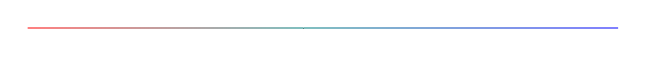
\begin{tikzpicture}
	\fill [left color=red!50, right color=teal!50] (0,0) rectangle (3.5,.01);
	\fill [left color=teal!50, right color=blue!50] (3.5,0) rectangle (7.5,.01);
	\end{tikzpicture}
\vspace{0.5cm}

\begin{theorem}[ Recta que pasa por dos puntos]

	\normalsize{La} ecuación de la recta que pasa por dos puntos $P(x_0,y_0) \text{ y } Q(x_1,y_1)$ tiene por ecuación:
	
	$$r:\ \begin{cases} \ P \\ \ Q \end{cases} \ \equiv \ \begin{cases} \ P \\ \ \vec v_r=\overrightarrow{PQ} \end{cases} \quad \Rightarrow \quad   \boxed{ \ \boldsymbol{ \dfrac{x-x_0}{x_1-x_0} \ = \ \dfrac{y-y_0}{y_1-y_0} } \ }$$
\end{theorem}
$r:\ \begin{cases} \ P \\ \ Q \end{cases} \ \equiv \ \begin{cases} \ P(x_0,y_0) \\ \ \vec v_r=\overrightarrow{PQ}=(x_1-x_0,y_1-y_0) \end{cases} \ \to \ $ en forma continua, $\ \dfrac{x-x_0}{x_1-x_0} \ = \ \dfrac{y-y_0}{y_1-y_0} $\QED


\vspace{5mm}
\begin{miejemplo}

Comprueba que pos puntos $P_1(-3,4),\ P_2(-1,5)  \text{ y }	 P_3(1,6)$ están alineados.

\vspace{6mm} Este ejercicio aprendimos a resolverlo en el apartado anterior de 'Sistema de Referencia', bata con comprobar que $\overrightarrow{P_1P_2}$ es paralelo (tiene la misma dirección) que $\overrightarrow{P_1P_3}$. Basta para ello con formar los vectores y comprobar que sus componentes son proporcionales. En esta ocasión veremos un método alternativo, aunque más largo.

\vspace{2mm} Primero buscaremos la recta $r$ que pasa por los puntos $P_1$ y $P_2$ y luego comprobaremos si $P_3 \in  r:\ \begin{cases}  \ P_1 \\ \ P_2 \ \end{cases}\ \equiv \ \begin{cases}  \ P_1 \\ \ \vec v_r=\overrightarrow{P_1P_2} \ \end{cases}
 \to \ \begin{cases}  \ P_1(-3,4) \\ \ \vec v_r=P_2-P_1=(2,1) \ \end{cases} \Rightarrow   \ r:\  \dfrac{x+3}{2}=\dfrac{y-4}{1}$

\vspace{2mm} Recta que en forma general (p.e.) se expresa como $x-2y+11=0$. Veamos si $P_3 \in r$, para ello sustituiremos las coordenadas de $P_3$ en la ecuación de $r$ y, si se satisface la ecuación, $P_3 \in r$  y si no se cumple, $P_3 \notin r \, : \qquad P_3(1,6) \ \to \ (1)-2(6)+11 = 0 \, , \ $  sí se verifica la ecuación por lo que $P_3\in r$ y los tres puntos están alineados.
\end{miejemplo}

\vspace{5mm}

\begin{cuadro-naranja}
\underline{!`Atención!}:

$\triangleright \quad $ Si la recta viene dada en forma paramétrica, $\begin{cases} \ x=a+kv_1\\ \ y=b+kv_2 \end{cases} $ rápidamente un punto por donde pasa es el $P(a,b)$ y un vector director el $\vec v=(v_1,v_2)$, los coeficientes que multiplican al parámetro.	

$r: \ \begin{cases} \ x=-2+k \\ \ y=3-2k \end{cases} \ \to \ \begin{cases} \ P_r(-2,3) \\ \ \vec v_r=(1,-2) \end{cases}\ ; \qquad \qquad 
s: \ \begin{cases} \ x=3 \\ \ y=k \end{cases} \ \to \ \begin{cases} \ P_s(3,0) \\ \ \vec v_s=(0,1) \end{cases}$

\vspace{4mm} $\triangleright \quad $ Si la recta viene dada en forma continua, $\dfrac{x-a}{v_1}=\dfrac{y-b}{v_2}$, el punto directamente lo obtenemos de los números que restan a las incógnitas en los numeradores, $P(a,b)$ y el vector como los números de los denominadores, $\vec v=(v_1,v_2)$.

\begin{small}
$r:\ \dfrac{x-3}{5}=\dfrac{y+7}{-2} \ \to \ \begin{cases} \ P_r(3,-7) \\ \ \vec v_r=(5,-2) \end{cases}  \qquad   s:\ \dfrac{2-x}{3}=\dfrac{2y+1}{4} \ \equiv \  \dfrac{x-2}{-3}=\dfrac{y+1/2}{4/2} \ \to \ \begin{cases} \ P_r(2,-1/2) \\ \ \vec v_r=(-3,2) \end{cases}$ \end{small}

\vspace{4mm} $\triangleright \quad $ Si una recta viene dada en forma punto pendiente, $y-b=m(x-a)$, un punto por donde pasa es $P(a,b)$, siendo $m$ la pendiente. $\quad [ \ y+2=-3(x-1)$ pasa por $P(1,-2) \ $ con pendiente $m=-3\ ]$


\vspace{4mm} $\triangleright \quad $ Si una recta viene dada en forma explícita,  $y=mx+n$, \textcolor{gris}{(lo enseña todo \smiley )} directamente se obtiene la pendiente (inclinación) como el coeficiente que multiplica a la $x$ y la ordenada en el origen (corte con eje $Y$) como el término independiente, !`ojo!, la $y$ debe estar despejada, sola en un miembro de la ecuación, por tratarse  de la ecuación explícita. $[\, y=2x+5 \ $ tiene pendiente $m=2$ y ordenada en el origen $n=5 \, ]$


\vspace{4mm} $\triangleright \quad $ Si una recta viene dada en forma general, $Ax+By+C=0$, el vector asociado (perpendicular) a la recta es $\vec n=(A,B)$. Por ello, un vector director de la recta sería en $\vec v=(-B,A)$ \textcolor{gris}{$ (\ \vec n \perp \vec v \ )$} $\quad [ \ 2x-3y+4=0 ;\quad \to \quad  \vec n=(2,-3);\ \vec v=(3,2) \quad \textcolor{gris}{ (\ \vec n \perp \vec v \ \leftrightarrow \ \vec n \cdot \vec v=0 \ ) } \  ]$

\vspace{6mm} \emph{Para pasar de una ecuación a otra de una recta, si no es directo, siempre se pueden buscar dos puntos de la recta y tomar uno de ellos como punto por donde pasa y con el otro formar un vector director.}
\end{cuadro-naranja}



\vspace{5mm}
\subsection{Haz de rectas}
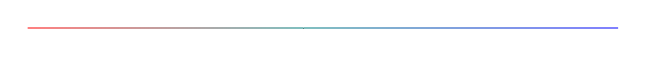
\begin{tikzpicture}
	\fill [left color=red!50, right color=teal!50] (0,0) rectangle (3.5,.01);
	\fill [left color=teal!50, right color=blue!50] (3.5,0) rectangle (7.5,.01);
	\end{tikzpicture}
\vspace{0.5cm}


\begin{definition}[ Haz de rectas concurrentes]

Al conjunto de todas las rectas que pasan por el punto $P(x_0,y_0)$ se le llama \emph{haz de rectas} concurrentes de \emph{vértice} $(x_0,y_0)$. Su expresión analítica es $\quad \boldsymbol{k(x-x_0)+k'(y-y_0)=0}$
	
\end{definition}

\underline{Observaciones}:

\begin{itemize}
	\item Al dar valores a los parámetros $k$ y $k'$, no simultáneamente nulos, se obtienen las rectas del haz.
	\item Si $k=0 \ \wedge \ k'=1 \ \to \ y=y_0\, , \ $, recta horizontal del haz.
	\item Si $k=1 \ \wedge \ k'=0 \ \to \ x=x_0\, , \ $, recta vertical del haz.
	\item Si lo que se conocen son las ecuaciones (generales) de dos de las rectas del haz, $\ r:	\ ax+by+c=0\ $ y $\ s:\ a'x+b'y+c'=0 \ $ la ecuación del haz es: $\ k(ax+by+c)+k'(a'x+b'y+c')=0$
	\item Si el haz viene dado en forma explícita, $\ y-y_0=m(x-x_0)\ $ \textcolor{gris}{(para cada valor de $m$ se obtiene una recta del haz)}, falta añadir la recta vertical $\ x=x_0$
\end{itemize}

\vspace{5mm}
\begin{theorem}[ Haz de rectas paralelas]

La ecuación de todas las rectas paralelas a la recta $r:\ Ax+By+C=0$ es de la forma: $\quad \boldsymbol{Ax+By+K=0}\, , \ \ \forall k\in \mathbb R$	
\end{theorem}

\underline{Demostración}: La recta $r$ tiene por vector director $\vec v_r=(-B,A)$, el mismo que todas las rectas del haz. Luego son todas paralelas. \QED

\vspace{0.5cm}
\begin{figure}[H]
	\centering
	\includegraphics[width=.75\textwidth]{img-ga/ga17.png}
	\caption*{\footnotesize{\textcolor{gris}{Haz de rectas.}}}
\end{figure}
\vspace{5mm}
\begin{miejemplo}

Escribe la ecuación de todas las rectas que pasan por el punto $P(2,1)$. ?`Cuál de ellas pasa por el punto $Q(0,3)$?	 ?`Y por el punto $R(2,-3)$? ?`Cuál de ellas es paralela al la recta $s:\ x+2y=5$?

\vspace{6mm} $\triangleright \quad $ \underline{En forma explícita}, el haz de vértice $P(2,1)$ tiene por ecuaciones: $\ y+1=m(x-2)\, , \ \forall m\in \mathbb R$ y la recta vertical $x=2$

\vspace{4mm} $\triangleright \quad $ Para encontrar cual de estas rectas pasan por $Q(0,3)$, sustituiremos las coordenadas de $Q$ en las ecuaciones del haz:
$3+1=m(0-2) \ \to \ 4=-2m \ \to \ m=-2 \ \Rightarrow \ y+1=-2(x-2)$

\vspace{4mm} $\triangleright \quad $  Para encontrar cual de estas rectas pasan por $R(2,-3)$, sustituiremos las coordenadas de $Q$ en las ecuaciones del haz:
$-3+1=m(2-2) \ \to \ -2=0\, m \ \to \ \nexists m \ \Rightarrow \ $ solo nos queda una recta del haz, la vertical: $\ x=2$ que evidentemente pertenece al haz de rectas que pasan por $P(2,1)$ y también pasa por $R(2,-3)$

\vspace{4mm} $\triangleright \quad $ la pendiente de la recta $s:\ 2y=-x+5 \ \to \ y=-\frac 1 2 x + \frac 5 2 \ \to \ m_s=-\frac 12$. Como todas las rectas paralelas tienen la misma pendiente, ha de ocurrir que $r \parallel s \ \leftrightarrow \ m_r=m_s=-\frac 1 2\, , \ $ por lo que la recta buscada será $\ y+1=-\dfrac 1 2 (x-2)$, simplificando, $\ y=-\dfrac 1 2 \, x$

\vspace{8mm} $\checkmark \quad $ Si preferimos trabajar  \underline{en forma general}, la ecuación del haz es $\ k(x-2)+k'(y+1)=0$

\vspace{2mm} $\checkmark \quad $ $Q(0,3) \ \to \ k(0-2)+k'(3+1)=-2k+4k'=0 \ \to \ k=2k'$ Esta es la relación que deben cumplir los parámetros $k\text{ y } k'$ del haz para elegir una de sus rectas y que pase por $P$. Por ejemplo, $k'=1 \text{ y } k=2 \ \to \ $ la recta buscada es $\ 2(x-2)+(y+1)=0$

\vspace{2mm} $\checkmark \quad $ $R(2,-3) \ \to \ k(2-2)+k'(-3+1)=-2k'=0 \ \to k'=0$. Bastará com dar a $k$ cualquier valor (distinto de cero, no pueden ser ambos parámetros simultáneamente nulos); por ejemplo, para $k=1 \ \to \ $ la recta buscada es $\ x-2=0$

\vspace{2mm} $\checkmark \quad \begin{cases} \text{ Haz: } kx+k'y-2k+k'=0 \\  \text{ s: } x+2y-5=0 \end{cases} \ \to \  $ Según los coeficientes, la recta del haz que es paralela a la recta $s$ es la que tiene $\ k=1 \ \wedge \ k'=2 \ \to \ x+2y-2(1)+2=0 \ \Rightarrow \ x+2y=0$ 
\end{miejemplo}

\vspace{5mm}

\begin{miejercicio}
	
	Encuentra la recta del haz de vértice $P(2,-1)$ que pasa por el origen de coordenadas.
	
	\rule{250pt}{0.1pt}
	
\vspace{2mm} Haz: $\ y+1=m(x-2)$, recta que pasa por $(0,0)\, : \quad 0+1=m(0-2) \ \to \ 1=-2m \ \to \quad  m=-\dfrac 1 2 \quad \Rightarrow \quad y+2=-\dfrac 1 2 \, (x-2) \ 	 \to \ \ y=-x$

\end{miejercicio}

\begin{miejercicio}
	
Sean $\ r:\ 3x+y-11=0$ y $\ s:\ x+2y-7=0$ Encuentra el haz que determinan y su vértice.
	
	\rule{250pt}{0.1pt}
	
\vspace{2mm}  Haz: $\ k(3x+y-11)+k'(x+2y-7)=0$

\vspace{2mm} Los pares $(x,y)$ que verifican la ecuación $3x+y-11=0$ son los infinitos puntos de esa recta. Análogamente, los pares $(x,y)$ que verifican la ecuación $x+2y-7=0$ son los infinitos puntos de la otra recta. El vérice del haz es punto de ambas rectas, será la intersección de ambas rectas, un punto $(x,y)$ que verifique simultáneamente ambas ecuaciones:
$\quad V(x,y) \ \begin{cases} \ 3x+y-11 &=0 \\ \ x+2y-7&=0 \end{cases} \ \to\ y=4 \ \wedge \ x=-1 \quad \Rightarrow \quad V(-1,4)$

\end{miejercicio}

\vspace{1cm}
\section{Posiciones relativas de dos rectas}

\begin{tikzpicture}
	\fill [left color=red!50, right color=teal!50] (0,0) rectangle (3.5,.1);
	\fill [left color=teal!50, right color=blue!50] (3.5,0) rectangle (7.5,.1);
	\end{tikzpicture}
\vspace{0.3cm}

Las posiciones relativas (sin atender a ángulos ni distancias) que pueden ocupar dos rectas en el plano son: 

$\checkmark \quad $ o son \subrayado{\text{paralelas}} y no tienen ningún punto en común, $\quad  \subrayado{\boxed{r \, \parallel \, s}}$

$\checkmark \quad $ o son \subrayado{\text{secantes, se cortan en un punto}} (que hay que determinar) que es el único común a las dos rectas, $\quad  \subrayado{\boxed{r \, \cap \, s \, = \, P} }$

$\checkmark \quad $ o son rectas \subrayado{\text{coincidentes}}, la misma recta,  con sus infinitos puntos en común, $\quad  \subrayado{\boxed{r \, \equiv \, s}}$

\begin{small}
\vspace{3mm} Si las rectas vienen dadas en forma continua o explícita nos preguntaremos si son o no paralelas (si tienen el mismo vector director o la misma pendiente). Si la respuesta es NO, entonces se tratará de rectas \underline{secantes} y tendremos que averiguar el punto de corte que, al ser común a ambas, encontraremos al resolver el sistema de ecuaciones formado por ambas rectas. Si la respuesta es SI, las rectas pueden ser paralelas o coincidentes, para discernir entre estos dos casos nos preguntaremos si un punto cualquiera de una de las rectas está en la otra recta (verifica su ecuación); si la respuesta es SÍ, tendremos dos rectas de la misma dirección con un punto en común, es decir, todos sus puntos han de ser comunes y se tratará de rectas \underline{coincidentes} (son la misma recta) ; si la respuesta es No, las rectas serán \underline{paralelas}, sin ningún punto común.

\vspace{3mm} Si las rectas vienen dadas en forma general, para encontrar qué tienen en común (cuestión que determinará sus posiciones relativas) resolveremos el sistema de ecuaciones formado por ambas rectas. Si el sistema resulta \underline{incompatible}, sin soluciones, tendremos rectas \underline{paralelas}. Si el sistema sí tiene solución, sistema compatible dependerá de si este es \underline{compatible determinado}, solución única, las rectas son \underline{secantes} (el punto de intersección es la solución del sistema) o \underline{compatible indeterminado}, infinitas soluciones, las rectas serán \underline{coincidentes}, se tratará de una sola recta (ambas son la misma) y la solución será la ecuación de cualquiera de ellas.
\end{small}

\vspace{3mm} Esquemáticamente:


\begin{theorem} [Posiciones relativas de dos rectas dadas en forma general]

$$\begin{cases} \ r:\ Ax+By+Cz&=0 \\ \\ \ s:\ A'x+B'y+C'z&=0 \end{cases} \qquad \Rightarrow \qquad  \begin{array}{llc} SCD & \to & r\cap s=P \\ \\ SCI &\to & r\equiv s \\ \\ SI &\to & r\parallel s \end{array}$$

\begin{center}
\rule{250pt}{0.1pt}	
\end{center}


$$\text{Más fácil } \qquad  \begin{cases} 
 \ \dfrac A{A'}=\dfrac{B}{B'}=(\to) 
 \begin{cases}
 \ (\to)=\dfrac{C}{C'} \ \to \ \text{ coincidentes}
 \\ \\
  \ (\to)\neq \dfrac{C}{C'} \ \to \ \text{ paralelas}
 \end{cases}
 \\ \\
 \ \dfrac A{A'} \neq \dfrac{B}{B'} \ \to \ \text{ secantes}	
 \end{cases}$$

\end{theorem}



\begin{theorem} [Posiciones relativas de dos rectas dadas en forma continua]

$$\begin{cases} \ r:\ P_r,\ \vec v_r \\ \\ \ s:\ P_s, \vec v_s \end{cases} \ \Rightarrow \ 
\text{?` } \vec v_r \, \parallel \, \vec v_s \text{\ ?} \ \to \
\begin{cases}
	\text{ Sí } 
\ \to \ \text{ ?`} \ P_r \in s \text{ ? } \ \to \
		\begin{cases}
		\text{ Sí}     &\to r\equiv s \text{ coincidentes}
		\\ \\ \text{ No } &\to r\parallel s \text{ paralelas}
		\end{cases}	
\\ \\ \text{ No }\ \to \ r\cap s=P \text{ secantes}
\end{cases}$$
	
\end{theorem}

\begin{theorem} [Posiciones relativas de dos rectas dadas en forma explícita]

$$\begin{cases} \ r:\ P_r,\ m_r \\ \\ \ s:\ P_s, \ m_s \end{cases} \ \Rightarrow \ 
\text{?` } m_r \, \parallel \, m_s \text{\ ?} \ \to \
\begin{cases}
	\text{ Sí } 
\ \to \ \text{ ?`} \ P_r \in s \text{ ? } \ \to \
		\begin{cases}
		\text{ Sí}     &\to r\equiv s \text{ coincidentes}
		\\ \\ \text{ No } &\to r\parallel s \text{ paralelas}
		\end{cases}	
\\ \\ \text{ No }\ \to \ r\cap s=P \text{ secantes}
\end{cases}$$
	
\end{theorem}

\vspace{5mm}
\begin{miejemplo}

Encuentra las posiciones relativas de las siguientes parejas de rectas.

\vspace{2mm} $a)\ \ r:\ \dfrac{x-1}{1}=\dfrac{y+2}{-1} \, ; \ \ s:\ \dfrac{x}{0}=\dfrac{y+2}{3};\qquad b) \ \  r:\ y=2x+5\, ;\ \ s:\ y=2x-1;\qquad $

\vspace{2mm} $c)\ \ r:\ y=2x+5\, ;\ \ s:\ \dfrac x 1 =\dfrac{y-5}{2}$	

\vspace{8mm} $\triangleright \ \ a)\quad P_r(1,-2),\ \vec v_r=(1,-1);\ \ p_s(0,-2),\ \vec v_s=(0,3) \quad \to \quad \vec v_r \, \not \parallel \, \vec v_s \ \to \ r\cap s=Q$

\vspace{2mm} $Q=r\cap s\ $ lo encontraremos al intersetar ambas rectas, resolver el sistema formado por ambas: $\ \ \begin{cases} \ r:\ -x+1=y+2 \\ \ s:\ y+2=0 \end{cases} \ \to \ y=-2 \ \wedge \ x= 1 \ \to \ r \text{ y } s $ se cortan en $(1,-2)$ 

\vspace{5mm} $\triangleright \ \ b)\quad m_r=m_s=2 \ \to \ r \text{ y } s $ son paralelas o coincidentes.  Tomemos un punto cualquiera de $r$, por ejemplo, si hacemos $x=0 \ \to \ y=2\cdot 0+5=5 \ \to \ P_r(0,5)$. Nos preguntamos si este punto verificará (pertenecerá a) la ecuación de la recta $s,\quad 5  \neq  2\cdot 0-1 \ \to \ P_r \notin s \ \to \ r\parallel s\, , \ $ las rectas son paralelas. 

\vspace{5mm} $\triangleright \ \ c)\quad m_r=2;\ \ \vec v_s=(1,2) \ \to \ m_s=\dfrac 2 1 =2=m_s \quad \to \ \ r \text{ y } s $ son paralelas o coincidentes. Tomado un punto de $r,\ P_r(0,5)$, al sustituirlo en la ecuación de $s,\ \ \dfrac{0}{1}=\dfrac{5-5}{2}$, sí se verifica la ecuación luego $P_r\in s$. Tenemos dos rectas paralelas con un punto en común, luego todos los puntos deben de ser comunes y tratarse de rectas $r\equiv s$, coincidentes. 
\end{miejemplo}


\begin{miejercicio}

Comprueba que las rectas, $\ \begin{cases} 2x+y-1=0 \\ x-y-2=0 \end{cases};\quad \begin{cases} 2x+y-1=0 \\ 2x+y-2=0 \end{cases};\quad  \begin{cases} 2x+y-1=0 \\ 4x+2y-2=0 \end{cases}\ $ son, respectivamente, secantes en (1,-1), paralelas y coincidentes.

\rule{250pt}{0.1pt}

\vspace{2mm} Algebraicamente, tan solo hay que resolver los sistemas y comprobar que el primero es SCD con solución $x=1,\ y=-1$, que son las coordenadas del punto de corte (o intersección); que el segundo sistema es SI y el tercero SCD.	

\begin{footnotesize}
\vspace{5mm} $\checkmark\quad$ De otro modo, atendiendo a los coeficientes de las rectas expresadas en forma general, en el primer caso $\dfrac{2}{1} \neq \dfrac{1}{-1} \ \to \ $ secantes. Al resolver el sistema se encontrará que el punto de intersección (corte) de ambas rectas será el (1,-1)

\vspace{3mm} $\checkmark\quad \dfrac{2}{2}=\dfrac{1}{1}\neq\dfrac{-1}{-2} \ \to \ $ rectas paralelas.
$\qquad \qquad $
$\checkmark\quad \dfrac{2}{4}=\dfrac{1}{2}=\dfrac{-1}{-2} \ \to \ $ rectas  coincidentes.
\end{footnotesize}
\end{miejercicio}





\vspace{0.5cm}
\section{Paralelismo y perpendicularidad}

\begin{tikzpicture}
	\fill [left color=red!50, right color=teal!50] (0,0) rectangle (3.5,.1);
	\fill [left color=teal!50, right color=blue!50] (3.5,0) rectangle (7.5,.1);
	\end{tikzpicture}
\vspace{0.2cm}


\begin{table}[H]
\centering
\begin{tabular}{ll|ccc}
Ecuación &  & $\ $ vector director & pendiente & vector normal \\ &&&& \\ \hline &&&& \\
Paramétricas & $\begin{cases} \, x=x_0+kv_x \\ \, y=y_0+kv_y \end{cases}$ & $(v_x,v_y)$  & $\dfrac {v_y}{v_x}$ & $(-v_y,v_x)$ \\ &&&& \\
Continua & $\dfrac{x-x_0}{v_x}=\dfrac{y-y_0}{v_y}$ & $(v_x,v_y)$  & $\dfrac {v_y}{v_x}$ & $(-v_y,v_x)$ \\ &&&& \\
Implícita & $Ax+By+C=0 \ $  & $(-B,A)$ & $-\dfrac A B$ & $(A,B)$ \\ &&&& \\
Explícita & $y=mx+n$ & $(1,m)$ & m & $(m,-1)$
\end{tabular}
\end{table}

\vspace{5mm}
\begin{theorem}[ Condiciones de paralelismo y perpendicularidad]

\begin{large}
$$ \boxed{ \ \boldsymbol{ r\, \parallel \, s \quad \Leftrightarrow \quad  \vec v_r\, \parallel \, \vec v_s \quad \Leftrightarrow \quad \dfrac{A}{B}=\dfrac{A'}{B'} \quad \Leftrightarrow \quad m_r\, = \, m_s } \ } $$	

$$ \boxed{ \ \boldsymbol{ r\, \perp \, s \quad \Leftrightarrow \quad  \vec v_r \cdot  \vec v_s=0 \quad \Leftrightarrow \quad AA'+BB'=0 \quad \Leftrightarrow \quad  m_r\, m_s \ = \ -1} \ } $$	
\end{large}
\end{theorem}

\underline{Demostración}:

\begin{itemize}
\item Obviamente, dos rectas son paralelas si tienen los mismos (o paralelos) vectores directores, por lo que sus pendientes serán iguales: 

$ \vec v_r=(v_x,v_y) \ \to \ \vec v_s=k\vec v_r=(kv_x,kv_y) \ \ \Rightarrow \ \ m_r=\dfrac{v_y}{v_x}=\dfrac{kv_y}{kv_x}=m_s$
\item Dos rectas serán perpendiculares si lo son sus vectores directores:

$r\perp s \ \leftrightarrow \ \vec v_r \perp \vec v_s \quad \Leftrightarrow \quad \vec v_r\cdot \vec v_s= 0 \quad \Leftrightarrow \quad v_{rx}v_{sx}+v_{ry}v_{sy}=0 \ \to $

$\to \ v_{rx}v_{sx}=-v_{ry}v_{sy} \ \to \ -\dfrac{v_{rx}}{v_{ry}}=\dfrac{v_{sy}}{v_{sx}} \ \Rightarrow \ m_s=-\dfrac{1}{m_r} \qquad \textcolor{gris}{(\, m_r\, m_s=-1 \, ) }$ \QED
  \end{itemize}


\vspace{5mm}

\begin{miejercicio}

Encuentra una recta paralela y otra perpendicular a la recta $r:\ 6x-3y-12=0	$ que pasen por el punto $P(2,-1)$

\rule{250pt}{0.1pt}

\vspace{2mm} \underline{En forma general}, 

\vspace{2mm} $s\parallel r \, : \ \ 6x-3y+k=0$ Determinaremos $k$ exigiendo que esta recta pase por $P(2,-1)$, que verifique su ecuación:

\vspace{2mm} $6(2)-3(-1)+k=0 \ \to \ 15+k=0 \ \to \ k=-15 \quad \Rightarrow \quad s:\ 6x-3y-15=0 \, \parallel \, r$

\vspace{4mm} $t\perp s \, : \ \ 3x+6y+k=0$ Determinaremos $k$ exigiendo que esta recta pase por $P(2,-1)$, que verifique su ecuación:

\vspace{2mm} $3(2)+6(-1)+k=0 \ \to \ k=0 \quad \Rightarrow \quad t:\ 3x+6y=0 \, \perp r$

\vspace{8mm}  \underline{En forma explícita},

\vspace{2mm} $r:\ y=2x-4 \ \to \ s \parallel r:\ \ y=2x+n$ Determinaremos $n$ exigiendo que $s$ pase por $P(2,-1) \ \to \ -1=2(2)+n \ \to \ n=-5 \quad \Rightarrow \quad s:\ y=2x-5 \, \parallel r$

\vspace{4mm} $r:\ y=2x-4 \ \to \ t \perp r:\ \ y=-\frac 12x+n$ Determinaremos $n$ exigiendo que $s$ pase por $P(2,-1) \ \to \ -1=-\frac 1 2(2)+n \ \to \ -1=-1+n \ \to \  n=0 \quad \Rightarrow \quad t:\ y=-\dfrac 1 2\, x \, \perp r$
\end{miejercicio}


\begin{miejercicio}

Sean $\ r:\ ax-2y+7=0 \ \text{ y } \ s:\ \dfrac{x+1}{b}=\dfrac{y}{2}$

\vspace{2mm} Determina el valor de $a$ y $b$ sabiendo que las rectas son perpendiculares y que $r$ pasa por el punto $P(1,2)$

\rule{250pt}{0.1pt}

\vspace{2mm} $r:\ 2y=ax+7 \ \to \ y=\dfrac a 2 \, x+ \dfrac 7 2 \ ; \quad m_r=\dfrac a 2$

\vspace{2mm} $s:\ 2x+2=by \ \to \ y=\dfrac 2 b \, x + \dfrac 2 b \ ; \quad m_s=\dfrac 2 b$

\vspace{2mm} $r\perp s \ \leftrightarrow \ m_r\, m_s=-1 \ \to \ \dfrac a 2 \dfrac 2 b =-1 \ \to \ \dfrac a b= -1\ \ (1*)$

\vspace{2mm} $P(1,2)\in r \ \to \ 	a(1)-2(2)+7=0 \ \to \ \boldsymbol{ a=-3} \ \ (2*)$

\vspace{2mm} Llevando el resultado $(2*)$ a la condición $(1*)$, $\quad \dfrac {-3} {b}=-1 \ \to \ \boldsymbol{b=3}$
\end{miejercicio}


\begin{miejercicio}

Sean $\ r:\ 5x-y+4=0\ \text{ y } \ s:\ \begin{cases} \ x&=-3+m\, k \\ \ y&=4-k \end{cases}$

\vspace{2mm} Determina el valor de $m$ para que las rectas sean $\ $ a) paralelas, b) perpendiculares y c) coincidentes.

\rule{250pt}{0.1pt}



\vspace{2mm} $s:\ \dfrac{x+3}{m}=\dfrac{y-4}{-1} \ \to \ -x-3=my-4m \ \to \ 
x+my-4m+3=0$


\vspace{4mm} $\triangleright \ \ a) \text{ y } c) \quad r\parallel s \ \leftrightarrow \ \dfrac{A'}{A}=\dfrac{B'}{B} \neq \dfrac{C'}{C} \ \to \ \dfrac{1}{5}=\dfrac{m}{-1} \ \leftrightarrow \ m=-\dfrac 1 5 $

\vspace{2mm} $r$ y $s$, de momento, serán paralelas $(r\parallel s)$ o coincidentes $(r\equiv s)$. Falta comprobar que $\dfrac 1 5 \neq \dfrac{C'}{C}=\dfrac{-4m+3}{4}=\dfrac{-4\frac {-1}{5} +3}{4}=\dfrac{19}{20}$ que sí se cumple la relación, por lo que para $m=-\dfrac 1 5  \ \Rightarrow \ r\parallel s$ y $\nexists m\ / \ r\equiv s$ 

\vspace{4mm} $\triangleright \ \ b) \quad r\perp s \ \leftrightarrow \ AA'+BB'=0 \ \to \ 5(1)-1(m)=0 \ \to \ m=5$


\end{miejercicio}



\vspace{1cm}
\section{Problemas métricos: ángulos y distancias}

\begin{tikzpicture}
	\fill [left color=red!50, right color=teal!50] (0,0) rectangle (3.5,.1);
	\fill [left color=teal!50, right color=blue!50] (3.5,0) rectangle (7.5,.1);
	\end{tikzpicture}
\vspace{0.5cm}

\subsection{Ángulos}
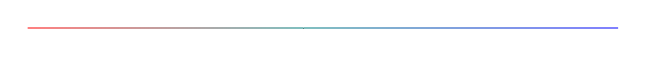
\begin{tikzpicture}
	\fill [left color=red!50, right color=teal!50] (0,0) rectangle (3.5,.01);
	\fill [left color=teal!50, right color=blue!50] (3.5,0) rectangle (7.5,.01);
	\end{tikzpicture}
\vspace{0.5cm}

\begin{figure}[H]
	\centering
	\includegraphics[width=.75\textwidth]{img-ga/ga18.png}
\end{figure}

Definiremos el ángulo entre dos rectas como el menor de los dos que forman. Si estos son $\theta_1$ y $\theta_2$, como se observa en la figura, son suplementarios, tienen cosenos opuestos. 

El ángulo que forman dos vectores puede ser cualquiera entre $0^o$ y $180^o$, esto depende de la orientación de los mismos como también se representa en la figura. Si el ángulo es mayor de $90^o$, su coseno será negativo ($\theta_2$), pero tomando valor absoluto tendremos coseno positivo y ángulo menor de $90^o$ $\, (\theta_1)$. 

Usaremos este resultado para definir el ángulo entre dos rectas como el que forman sus vectores directores pero considerando el valor absoluto de su producto escalar:

\vspace{5mm}
\begin{definition}[ Ángulo entre dos rectas (a partir de sus vectores directores)]

Se define el ángulo entre dos rectas como el menor de los dos que forman	, él ángulo menor de $90^o$, por ello, 

$$\theta_{rs} \ = \ \measuredangle (r,s) \ = \ \acos\ \dfrac{|\vec v_r \cdot \vec v_s|}{|\vec v_r| \, |\vec v_s|}$$

\begin{small}\textcolor{gris}{el módulo del valor absoluto del producto escalar de los vectores directores de las rectas nos asegura quedarnos con el menor de los dos ángulos que forman las rectas.}\end{small}
\end{definition}

\vspace{5mm}
\begin{definition}[ Ángulo entre dos rectas (a partir de sus vectores normales)]

\begin{multicols}{2}

$\ $

Puesto que dos ángulos que tienen los lados perpendiculares son iguales, 

$$\theta_{rs} \ = \ \acos\ \dfrac{|\vec n_r \cdot \vec n_s|}{|\vec n_r| \, |\vec n_s|}$$

\begin{figure}[H]
	\centering
	\includegraphics[width=.3\textwidth]{img-ga/ga19.png}
\end{figure}
\end{multicols}
\end{definition}

\underline{Observación}: El ángulo que forman dos rectas es el que forman sus vectores directores (o sus vectores normales) o su suplementario en caso de que éste sea mayor de $90^o$. Para obviar esta situación tomamos el valor absoluto del producto escalar.

\begin{theorem}[ Ángulo formado por dos rectas a partir de sus pendientes] 

	$$\begin{cases} \ r:\ y=m_1x+n \\ \ s:\ y=m_2+n_2 \end{cases} \quad \Rightarrow \qquad \theta_{rs} \ = \ \atan \ \left| \dfrac{m_1-m_2}{1+m_1\, m_2}  \right| $$
\end{theorem}

\begin{multicols}{2}
\underline{Demostración}:

De la figura, $\ \theta=\theta_1-\theta_2 \ \to $

$\to \ \ \tan \theta = \tan(\theta_1-\theta_2)= \dfrac{\tan \theta_1-\tan \theta_2}{1+\tan \theta_1\, \tan \theta_2}$

Como $\ m_1=\tan \theta_1 \ $ y $\ m_2=\tan \theta_2$ y teniendo en cuenta que el ángulo entre dos rectas es el menor de los dos ángulos que forman, obtenemos:
$\quad \tan \theta \ = \ \left| \dfrac{m_1-m_2}{1+m_1\, m_2} \right|$ \QED
\begin{figure}[H]
	\centering
	\includegraphics[width=.4\textwidth]{img-ga/ga20.png}
\end{figure}
\end{multicols}
\vspace{5mm}

\begin{miejemplo}

Calcula el ángulo que forman los siguientes pares de rectas:	

\vspace{2mm} $a)\ \ \begin{cases} \ \begin{cases} \ x=3-2t\\ \ y=7+t \end{cases} \\ \ \dfrac{x-1}{-4}=\dfrac{y-4}{3} \end{cases} \, ; \qquad b)\ \ \begin{cases} \ x+2y-17=0 \\ \ 3x-5y+4=0 \end{cases}\, ; \qquad c)\ \ \begin{cases} \ y=5x+3 \\ \ y=-2x+5 \end{cases}$

\vspace{6mm} $\triangleright \ \ a) \quad \vec v_1=(-2,1);\ \vec v_2=(-4,3) \ \to \ \cos \theta=\dfrac{|8+3|}{\sqrt{5}\, 5}=\dfrac{7}{5\sqrt{5}} \ \to \ \theta=10.3^o$


\vspace{5mm} $\triangleright \ \ b) \quad \vec n_1=(1,2);\ \vec n_2=(3,-5) \ \to \ \cos \theta = \dfrac{|3-10|}{\sqrt{5}\, \sqrt{34}}=\dfrac{7}{\sqrt{170}} \ \to \ \theta= 57.5^o$


\vspace{5mm} $\triangleright \ \ c) \quad m_1=5;	 m_2=-2 \ \to \ \tan \theta= \left| \dfrac{5-(-2)}{1+5(-2)} \right|=\dfrac{7}{9} \ \to \ \theta=37.9^o$

\end{miejemplo}

\vspace{5mm}
\begin{miejercicio}

Encuentra la ecuación de la recta $r$ que pasa por $P(2,-3)$ y forma un ángulo de $45^o$ con la recta $s:\ y=3x+3$

\rule{200pt}{0.1pt}

\vspace{2mm} $r:\ y+2=m(x-2)\, ; \ \theta(r,s)=45^o;\ m_1=m;\ m_2=3 \ \to \ \tan \theta=\left| \dfrac{m-3}{1+3m} \right|=\tan 45^o =1 \ \to $ 	

\vspace{2mm} $\tan \theta=\left| \dfrac{m-3}{1+3m} \right|=1 \to \ \begin{cases}
 \ 	\dfrac{m-3}{1+3m} =1 &\to \ m-3=3m+1 \ \to \ -2=2m \ \to \ m=-1
 \\
 \ \dfrac{m-3}{1+3m} =-1 &\to \ m-3=-3m-1 \ \to \ 4m=2 \ \to \ m=1/2
 \end{cases}$
 
 \vspace{2mm} Hay dos rectas que cumplen las condiciones: $ \ y+2=-(x-2) \ \ \wedge \ \ y+2=1/2(x-2)$

\end{miejercicio}


\vspace{5mm}
\subsection{Distancias}
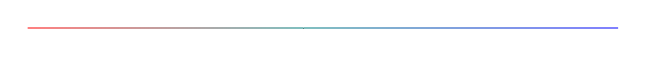
\begin{tikzpicture}
	\fill [left color=red!50, right color=teal!50] (0,0) rectangle (3.5,.01);
	\fill [left color=teal!50, right color=blue!50] (3.5,0) rectangle (7.5,.01);
	\end{tikzpicture}
\vspace{0.5cm}

Ya sabemos calcular la \textbf{distancia entre dos puntos}, $\ \boldsymbol{ \d(P,Q)=|\overrightarrow{PQ}| } \, ,. \ $ Vamos ahora a calcular la distancia de una recta a un punto y la distancia entre rectas.

\vspace{5mm}
\begin{large}
\textbf{Distancia de un punto $\boldsymbol{P(x_0,y_0)}$ a una recta $\boldsymbol{r}$}:	
\end{large}

\vspace{3mm}
\begin{definition}[ Proyección ortogonal]

\begin{multicols}{2}
Se difine la distancia de un punto $P(x_0,y_0)$ a una recta $r:\ Ax+By+C=0$ como	 la menor de todas las posibles. 

 Se trata de encontrar un punto de la recta, $Q\in r$, de modo que $d(P.Q)$ sea mínima. Es obvio que esto ocurrirá cuando $\overrightarrow{PQ} \, \perp \, \vec v_r$, y tendremos dos métodos para su cálculo.
\begin{figure}[H]
	\centering
	\includegraphics[width=.45\textwidth]{img-ga/ga21.png}
\end{figure} \end{multicols}

De todos los posibles puntos $Q\in r$, el que hace que la distancia al punto $P$ sea mínima es el \emph{``punto que está enfrente''}, se le llama \textbf{\emph{proyección ortogonal de $\boldsymbol P$ sobre $\boldsymbol r$}}.
\end{definition}

\vspace{5mm}
\begin{theorem}[ Algoritmo para el cálculo de la distancia de un punto a una recta]

Dado $P(x_0,y_0\ )$ y $\ r:\, Ax+By+C=0\, , \ $ para el cálculo de la distancia de $P$ a $r$ procederemos del siguiente modo:

\begin{enumerate}
\item Buscaremos la recta $s$, que siendo perpendicular a $r$ pase por el punto $P$


\item Calculamos la intersección de ambas rectas, que proporcionará el punto de $r$ que está \emph{frente} a $P$, la \underline{proyección ortogonal} de $P$ sobre $r$, que denotaremos por $Q$


\item Por último, definiremos la distancia entre $P$ y $r$ como la distancia entre $P$ y su proyección ortogonal sobre $r$, $Q$

$$\boldsymbol{ 1)\ \ s\,:\  \begin{cases} \ P(x_0,y_0) \\ \ \perp 	\, r \end{cases} \quad \qquad 2)\  \ Q\, = \ r\, \cap \, s  \quad \qquad 3)\ \ d(P,r) \ = \ d(P,Q) }$$

\item \textcolor{NavyBlue}{Este método nos proporciona de forma inmediata el punto \textbf{simétrico de un punto respecto de un a recta}, $P'$ ha de ser tal que la proyección ortogonal, $Q$ sea el punto medio del segmento $\overline{PP'}$}

$$\textcolor{NavyBlue}{P' \ / \ \dfrac{P+P'}{2}=Q}$$

\textcolor{NavyBlue}{$P'$ simétrico de $P$ respecto de $r$. $Q$ es la proyección ortogonal de $P$ sobre $r$.}
  	
\end{enumerate}

	
\end{theorem}


\textcolor{gris}{Recordemos que el simétrico de un punto $P$ respecto de un punto $Q$, será un punto $P'$ tal que el punto medio de $\overline{PP'}$ sea $Q$. Ahora hemos aprendido a calcular el simétrico de un punto $P(x_0,y_0)$ respecto de u a recta $r:\, Ax+By+C=0$ a partir de su proyección ortogonal.}

\vspace{5mm}
\begin{definition}[ Simétrico de una recta respecto de otra]

\begin{multicols}{2}	
	$r': \ $ simétrica de $r$ respecto de $s$ será la recta que pasa por los puntos $P'_r$ simétrico de $P_r$ respecto de $s$ y 	$Q'_r$ simétrico de $Q_r$ respecto de $s$, cualesquiera que sean los puntos $P_r$ y $Q_r$ de la recta $r$.

\vspace{2mm} Si las rectas son secantes, se puede tomar el punto de intersección como punto de la recta $r$ y su simétrica $r`$, $P_r=P'_r=r\cap s$ 
\begin{figure}[H]
	\centering
	\includegraphics[width=.45\textwidth]{img-ga/ga22.png}
\end{figure}
\end{multicols}
\vspace{-5mm} Si las rectas son coincidentes, cualquiera de las dos (son la misma) es la simétrica de una respecto de la otra.
\end{definition}

\vspace{5mm}
\begin{theorem}[ Fórmula para el cálculo de la distancia de un punto a una recta]

$$ P(x_0, y_0)\, ; \  \ r:\, Ax+By+C=0 \quad \to \qquad \boldsymbol{ d(P,r) \ = \ \dfrac{|Ax_0+By_0+C|}{\sqrt{A^2+B^2}} }$$	
\end{theorem}
\underline{Observaciones}:
\begin{itemize}
\item Para calcular la distancia de un punto a una recta basta con sustituir las coordenadas del punto en la ecuación general de la recta (todo a la izquierda igual a cero) y al resultado, en valor absoluto, dividirlo por el módulo del vector normal de la recta.
\item Este método no proporciona ni la proyección ortogonal del punto sobre la recta, ni el simétrico del punto respecto de la recta
\end{itemize}
\vspace{3mm} \underline{Demostración}:
\begin{multicols}{2}
$\begin{cases} \ P(x_0,y_0) \\ \ r:\, Ax+By+C=0 \end{cases} \ \to \ $ 

supongamos que $Q(q_x,q_y)\in r$ es el punto que está frente a $P$ en $r$ (proyección ortogonal), el que determina la distancia mínima. En estas condiciones,  que $d(P,r)=d(P,Q)$

Sabemos que $\overrightarrow{PQ} \perp r \ \to \ \overrightarrow{PQ} \perp \vec v_r \ \to \ \overrightarrow{PQ}\, \parallel \, \vec n_r$
\begin{figure}[H]
	\centering
	\includegraphics[width=.5\textwidth]{img-ga/ga23.png}
\end{figure}
\end{multicols}

Para facilitar los cálculos, tomaremos $\vec n_r$ como vector unitario: $\vec u_{\, n_r}=\dfrac 1{|\vec n_r|}\, \vec n_r=\dfrac{(A,B)}{\sqrt{A^2+B^2}}$

Como $\overrightarrow{PQ}\, \parallel \, \vec u_{\, n_r} \ \to \ \exists k\in \mathbb R \ / \ \overrightarrow{PQ}=k\, \vec u_{\, n_r}=k\, \dfrac{(A,B)}{\sqrt{A^2+B^2}}$,
siendo $|k|$ la distancia de $P$ a $r$, $\quad \boldsymbol{d(P,r)=|k|}$
	
Por una lado, $\ \overrightarrow{PQ} \cdot \vec u_{\, n_r}=k\, \vec u_{\, n_r}\cdot \vec u_{\, n_r}=\dfrac{(A,B)}{\sqrt{A^2+B^2}}\, \dfrac{(A,B)}{\sqrt{A^2+B^2}} =k\, 1 =k$

Por otro lado, al ser $\overrightarrow{PQ}=Q-P=(q_x-x_0,q_y-y_0) \ \to \ 
 \overrightarrow{PQ} \cdot \vec u_{\, n_r} = (q_x-x_0,q_y-y_0)\cdot \dfrac{(A,B)}{\sqrt{A^2+B^2}}= \dfrac{Aq_x-Ax_0+Bq_y-By_0}{\sqrt{A^2+B^2}}= (*)= \dfrac{-Ax_0-By_0-C}{\sqrt{A^2+B^2}}=k$
 
$(*):\ $  ya que $Q\in r \ to \ Aq_x+Bq_y+C=0 \ \Rightarrow \  Aq_x+Bq_y=-C$, por lo que

Como $\d(P,r)=|k| \quad \to \qquad \boldsymbol{ d(P,r) \ = \ \dfrac{|Ax_0+By_0+C|}{\sqrt{A^2+B^2}} }$ \QED




\vspace{5mm}
\begin{large}
\textbf{Distancia entre dos rectas $\boldsymbol{r}$ y $\boldsymbol{s}$}:	
\end{large}
\begin{theorem}[ Distancia entre dos rectas]

$$\boldsymbol{ \begin{array}{ccc}
r\equiv s \ \vee \ r\cap s & \longrightarrow & d(r,s)=0 \\ \\
r\, \parallel \, s & \longrightarrow & d(r,s)=d(P_r,s)=d(P_s,r)
\end{array} }$$
	
\end{theorem}

Si las rectas son secantes o coincidentes, la distancia (mínima) entre ellas es cero. Si son rectas paralelas, la distancia entre ellas es la misma que la distancia de un punto cualquiera de una de ellas a la otra recta.


\vspace{5mm}

\begin{miejemplo}

Calcula la distancia del punto $P(3,-2)$ a la recta $r:\, 3x+4y-5=0$ usando la fórmula.

\vspace{2mm} Repite el ejercicio usando el algoritmo y da también la proyección ortogonal y  y el simétrico de $P$ sobre $r$.

\vspace{8mm} \underline{Fórmula}: $\qquad d(P,r)=\dfrac{|3(3)+4(-2)-5|}{\sqrt{3^2+4^2}}=\dfrac{4}{5}\, \mathrm{u}$

\vspace{6mm} \underline{Algoritmo}: $\qquad 1)\ \  s:\ \begin{cases} \ P(3,2) \\ \ \perp r \to n_s=(-4,3) \end{cases} \ \to \ s:\, -4x+3y+k=0\, ; \ P\in s \ \to \ -4(3)+3(-2)+k=0 \ \to \ k=18 \ \Rightarrow \ s:\, -4x+3y+18=0$

\vspace{2mm} $2)\ \ r\cap s=Q \ \to \ \begin{cases} \ 3x+4y&=5 \\ \ -4x+3y&=-18 \end{cases} \ \to \  x=\dfrac{87}{25},\ y=-\dfrac{34}{25} \ \Rightarrow \ Q\left(\dfrac{87}{25},-\dfrac{34}{25} \right)$

\vspace{2mm} $3)\ \ \overrightarrow{PQ}=Q-P=\left(\dfrac{87}{25},-\dfrac{34}{25} \right)-(3,-2)=\left( \dfrac{12}{25}, \dfrac{16}{25} \right) \ \Rightarrow \  d(P,r)=|\overrightarrow{PQ}|=\sqrt{\left( \dfrac{12}{25} \right)^2 + \left( \dfrac{16}{25} \right)^2 }=\dfrac{\sqrt{4000}}{25}=\dfrac{20}{25}=\dfrac 4 5 \, \mathrm{u}$

\vspace{2mm} La proyección ortogonal de $P$ sobre $r$ la hemos obtenido en el paso 2), $\quad Q\left(\dfrac{87}{25},-\dfrac{34}{25} \right)$. Este punto ha de ser el punto medio de $P$ y $P'$, el simétrico de $P$ respecto de $r$, por lo que $\ \dfrac{P+P'}{2}=Q \ \to \ P'=2Q-P=2 \left(\dfrac{87}{25},-\dfrac{34}{25} \right)-(3,-2)=\left(\dfrac{174}{25},-\dfrac{68}{25} \right)-(3,-2)= \left( \dfrac{99}{25}, -\dfrac{18}{25} \right)$


\end{miejemplo}


%%%
\begin{miejercicio}

Encuentra el área del triángulo de vértices $A(-3,8)$, $B(-3,2)$ y $C(5,2)$ de tres formas distintas:

\begin{enumerate}[a) ]
\item Usando la fórmula de Heron.
\item Usando el producto escalar.
\item Usando la fórmula $\mathcal A=1/2 \, b\cdot h$, siendo $b=\overline{AC}$ y $h$ la distancia de $B$ a la recta que pasa por $AC$
\end{enumerate}


\rule{250pt}{0.1pt}

\vspace{2mm} --- Fórmula de Heron: $\qquad c=|\overrightarrow{AB}|=|(0,-6)|=\sqrt{0^2+(-6)^2}=6\, \mathrm{u};\quad b=|\overrightarrow{AC}|=|(8,-6)|=\sqrt{8^2+(-6)^2}=10\, \mathrm{u}; \quad a=|\overrightarrow{BC}|=|(8,0)|=\sqrt{8^2+0^2}=8\, \mathrm{u}$	

\vspace{2mm} $p=1/2(a+b+c)=12\, \mathrm{u} \ \Rightarrow \ \mathcal A=\sqrt{p(p-a)(p-b)(p-c)}=\sqrt{12\cdot 4\cdot 2\cdot 6}=24 \, \mathrm{u}^2$ 

\vspace{5mm} --- Producto escalar: $\qquad \overrightarrow{AB}\cdot \overrightarrow{AC}=|\overrightarrow{AB}|\, |\overrightarrow{AC}|\, \cos \theta \ \to \ ((0,-6)\cdot (8,-6)=36=6\, 10\, \cos \theta \ \to \ \theta=53.13^o \ \Rightarrow \ \mathcal A=1/2 |\overrightarrow{AB}|\, |\overrightarrow{AC}|\, \sin \theta =24\, \mathrm{u}^2$

\vspace{5mm} --- Usando la fórmula $\mathcal A=1/2 \, b\cdot h$, siendo $b=\overline{AC}$ y $h$ la distancia de $B$ a la recta que pasa por $AC$

\vspace{2mm} $\overline{AC}=|\overrightarrow{AC}|=10;\ \ r_{AC}:\,\begin{cases} A \\ B \end{cases} \equiv \begin{cases} A(-3,8) \\ \vec v_r=\overrightarrow{AB}=(8,-6) \end{cases} \ \to \ \dfrac{x+3}{8}=\dfrac{y-2}{-6} \ \Rightarrow \ r_{AB}:\, 3x+4y+1=0;\qquad h=d(B,r_{AC})=	\dfrac{| 3(-3) +4(8)+1|}{\sqrt{3^2+4^2}}=\dfrac{24}{5}\, \mathrm{u} \ \ \Rightarrow \ \ \mathcal A=1/2 \, 10\,  \dfrac{24}{5}=24 \, \mathrm{u}^2$
\end{miejercicio}

\begin{miejercicio}

Para el triángulo de vértices $A(2,1),\ B(4,-2),\ C(6,3)$, encuentra las ecuaciones de $\quad $ a) mediatriz del lado $AC$, $\ $ b) altura del vértice $A$, $\ $ c) mediana del lado $BC$

\rule{250pt}{0.1pt}

\vspace{2mm} $\checkmark\ $ \emph{Mediatriz de un segmento: recta perpendicular al segmento que pasa por su punto medio.}

\vspace{2mm} $mediatriz_{AC}: \ r:\, \begin{cases} M_{AC}=(A+C)/2=(4,2) \\  r \perp \vec{AC} =C-A=(4,2) \ \to v_r=(-2,4)\to (-1,2) \ (*) \end{cases}$

\vspace{2mm} $r:\ \dfrac{x-4}{-1}=\dfrac{y-2}{2} \ \to \  r:\, 2x+y-10=0$

\vspace{5mm} $\checkmark\ $ \emph{Altura (recta): en un triángulo es la recta perpendicular a un lado que pasa por el vértice opuesto}

\vspace{2mm} $altura_{A}:\ s:\, \begin{cases} A(2,1) \\ s\perp \overrightarrow{BC}=(2,5)\ \to \ v_s=(-5,2) \end{cases} \to \dfrac{x-2}{-5}= \dfrac{y-1}{2} \ \to \ s:\, 2x+5y-9=0$

\vspace{2mm} \color{NavyBlue}La altura del triángulo respecto del vértice $A$ es la distancia de ésta a la intersección de la recta anterior $s$ con la recta que pasa por $B$ y $C$, $r_{BC}$, punto $Q$. O, de otro modo, la distancia del punto $A(2,1)$ a la recta $r_{BC}$. Comprúebese, que en ambos casos, se obtiene una distancia igual a $16\sqrt{29}\, \mathrm{u}$.\color{Black}

\vspace{5mm} $\checkmark\ $ \emph{Mediana de un lado de un triángulo es la recta que pasa por el punto medio del lado y por el vértice opuesto}

\vspace{2mm} \begin{footnotesize}$mediana_{BC}:\ t:\, $  $\begin{cases} M_{BC}=(B+C)/2=(5,1/2) \\ A(2,1) \end{cases} \equiv \begin{cases} M(5,1/2) \\ \vec v_t=\overrightarrow{M_{BC}A}=A-M_{BC}=(-3,1/2) \to \ (6,-1) \ (*) \end{cases} $\end{footnotesize} 

\vspace{2mm} $t:\, \dfrac{x-5}{6}=\dfrac{y-1/2}{-1} \ \to \ t:\, x+6y-8=0$

\vspace{5mm} \textcolor{gris}{$(*)\ $ !`Los puntos no se pueden simplificar! \smiley{}  Los vectores tampoco, cambiaría su tamaño y, tal vez, su sentido. Pero los vectores directores sí se pueden simplificar, multiplicar o dividir por un número distinto de cero , siguen teniendo la misma dirección.}
  
\end{miejercicio}

%%%
\begin{miejercicio}

Calcula la ecuación de la recta $s$ que dista de la recta $r:\, 5x-12y+12=0$ una unidad.

\rule{250pt}{0.1pt}

\vspace{2mm} La recta buscada ha de ser paralela (secantes y coincidentes tiene distancia cero). 

$s:\, 5x-12y+k=0 \ \parallel r$ pues $\vec n_s\parallel \vec n_r$

\vspace{2mm} La distancia entre rectas paralelas coincide con la distancia entre un punto cualquiera de una de ellas a la otra recta y, para esto, disponemos de un fórmula que facilita el cálculo.

\vspace{2mm} $r:\, x=0 \ \to \ y=1 \ \Rightarrow \  P_r(0,1)\in r  \quad \Rightarrow \quad d(r,s)=d(P_r,s)=\dfrac{|5(0)-12(1)+k |}{\sqrt{5^2+(-12)^2}}=\dfrac{|k-12|}{13}=1 \quad \to \quad \begin{cases} \ \dfrac{k-12}{13}=1 &\to k=25 \\ \dfrac{k-12}{13}=-1 &\to k=-1 \end{cases}$

\vspace{2mm} Hay dos rectas que cumplen las condiciones del problema (dos soluciones): 

\vspace{2mm}$s_1:\ 5x-12y+25=0 \ \ \wedge \ \ s_2:\, 5x-12y+1=0$
	
\end{miejercicio}

%%%
\begin{miejercicio}

Calcula el simétrico de $A(6,3)$ respecto de $r:\, x+2y-2=0$

\rule{250pt}{0.1pt} 

\vspace{2mm}Utilizamos el algoritmo para el cálculo de la distancia de un punto a una recta. Al obtener como paso previo la proyección ortogonal de $P$ sobre $r$, el punto $Q$, aprovecharemos este resultado para exigir que $Q$ sea el punto medio de $\overline{AA'}$

\vspace{2mm} $1)\quad s:\, \begin{cases} \ A(6,3) \\ \perp r \to \vec n_s=(-2,1) \end{cases} \ \to \ -2x+y+k=0 \ / \ A(6,3)\in s \ \Rightarrow \ -2(6)+(3)+k=0 \ \to \ k=9 \quad \Rightarrow \quad s:\ -2x+y+9=0$

\vspace{2mm} $2)\quad Q=r\cap s = \begin{cases} x+2y=2 \\ -2x+y=-9 \end{cases} \ \to \ x=4 \, ; \ y=-1 \quad \Rightarrow \quad Q(4,-1)$

\vspace{2mm} $3) \quad d(A,r)=d(A,Q)$, no nos interesa en este problema.

\vspace{4mm} $4)\quad \dfrac{A+A'}{2}=Q \ \to \ A'=2Q-A=2(4,-1)-(6,3)=(2,-5)$

\end{miejercicio}

%%%
\begin{miejercicio}

a) Calcula la recta simétrica de $r:\, y=x+2$ respecto de la recta $s:\, y=2x$

\vspace{2mm} b) Calcula la recta simétrica de $r:\, y=x+2$ respecto de la recta $s:\, y=x+4$

\rule{250pt}{0.1pt}

\vspace{2mm} $\triangleright \ \ a)\quad $ Al tener las rectas distintas pendientes, serán secantes. Encontraremos primero el punto de corte, $R$, que será el punto común a ambas rectas.

\vspace{2mm} $R=r\cap s=\begin{cases} \ y=x+2 \\ \ y=2x \end{cases} \ \to \ x=2,\ y=4 \ \to \ R(2,4)$

\vspace{2mm} Ahora hemos de buscar un punto $P\in r$ para encontrar su simétrico respecto de la recta $s \ \to \ $ algoritmo (ejer. anterior). Sea éste, $P(0,2) \  \to   \ P'$, simétrico de $P$ respecto de $s$:

\vspace{2mm} $t:\ \begin{cases} \ P(0,2) \\ \ \perp s \to m_t=-1/2 \end{cases} \ \to \ t:\ y-2=-\dfrac 12 (x-2) \ \to \ t:\ y=-\dfrac 1 2 \, x+2$

\vspace{2mm} Proyección ortogonal de $P$ sobre $s$, punto $Q$ que será el punto medio de $PP'$: 

\vspace{2mm}$Q=s\cap t  = \begin{cases} \ y=2x \\ \ y=-\frac 1 2 x+2 \end{cases} \ \to \ x=4/5 \ \wedge \ y=8/5 \ \to \ Q(4/5,8/5)$

\vspace{2mm} El simétrico de $P\in r$ respecto de $s$ es $P'$ de modo que $Q$ sea el punto medio de $\overline{PP'}: \quad \dfrac{P+P'}{2}=Q \ \to \ P'=2Q-P=2(4/5,8/5)-(0,2)=(8/5,16/5)-(0,2)=(8/5,6/5)$

\vspace{2mm} Finalmente, la recta $r'$ buscada, simétrica de $r$ respecto de $s$ será la recta que pasa por los puntos $R$ (común a ambas rectas) y por $P'$ (simétrico de $P\in r$ respecto de $s$):

\vspace{2mm} $r':\,\begin{cases} R(2,4) \\ P'(8/5,6/5) \end{cases} \equiv \begin{cases} R(2,4) \\ \vec v_{r'}=\overrightarrow{RP}=(-2/5,-14/5) \ \to \ (-2,-14) \ \to \ (1,7) \ \Rightarrow \ m=7/1=7 \end{cases}$

\vspace{2mm} Finalmente, $\quad r':\ y-4=7(x-2) \ \Rightarrow \ y=7x-10$ 

\vspace{6mm} $\triangleright \ \ b)\quad $ Ahora, las rectas $r$ y $s$ son paralelas, por lo que también lo será la recta $r'$ buscada, simétrica de $r$ respecto de $s$.

\vspace{2mm} Deberíamos buscar dos puntos de la recta $r$ de los cuales buscar sus respectivos simétricos respecto de $s$ y ellos determinarían la ecuación de la recta $r'$ buscada. Pero veamos si podemos abreviar los cálculos: como hemos deducido que $r$ también será paralela a $r$ y a $s$, sabemos su pendiente, $m=1$. Solo necesitamos un punto por donde pasará, buscaremos pues un solo punto simétrico $P'$ de un punto $P\in r$ respecto de $s$ y, así, nuestra recta será $\ r'=\begin{cases} \, P' \\ \, m=1 \end{cases}$

\vspace{2mm}   Búsqueda de $P'$ simétrico de $P\in r$ respecto de $s$. Sea, por ejemplo, $P(0,2)\in r$

\vspace{2mm} $t:\ \begin{cases} P(0,2) \perp s \ \to \ m_t=-1/1=-1 \end{cases} \ \to \ y-0 =-1(x-2)  \ \to \ y=-x+2$

\vspace{2mm} $Q$, proyección ortogonal de $P$ sobre $s$, $\ Q=s\cap t = \begin{cases} y=x+4 \\ y=-x+2 \end{cases} \ \to \ Q(-1,3)$

\vspace{2mm} La proyección ortogonal de $P$ sobre $s$, $Q$, ha de ser el punto medio de $\overline{PP'} \quad  \to \quad P'=2Q-P=2(-1,3)-(0,2)=(-2,6)-(0,2)=(-2,4)$

\vspace{2mm} La recta $r'$ buscada es: $\ r':\ y=1\, x+n \ / \ P'(-2,4) \in r' \quad\Rightarrow \quad 4=1.(-2)+n \ \to \ n=6 \quad \Rightarrow \quad r':\ y=x+6$


\vspace{4mm} ------ De otro modo, busquemos la recta paralela a $s$ que diste de ella $d=d(r,s)$ unidades. Obtendremos 2 rectas que serán $r$ y $r'$, la recta buscada.

\vspace{2mm} $d=d(r,s)=d[\, P_r(0,2),s:\, x-y+4=0\, ] =\dfrac{|0-(2)+4|}{\sqrt{1^2+(-1)^2}}= \dfrac 2{\sqrt 2}=\sqrt{2}\, \mathrm{u}$

\vspace{2mm}$r,r':\ \parallel s \ / \ d(r',s)=\sqrt{2} \ \to \ \begin{cases} r':\, x-y+k=0 	\\ S\in s:\ S(0,4) \end{cases} \ \to \ \sqrt{2}=\dfrac{|0-(4)+k|}{\sqrt{1^2+(-1)^2}} \ \to \ 2=|k-4| \to \begin{cases} k-4=2 &\to k=6 \Rightarrow r' \\ k-4=-2 &\to k=2 \Rightarrow r \end{cases}$


\vspace{2mm} La recta buscada es $\ r':\ x-y+6=0 \ \leftrightarrow \ y=x+6$ 

\end{miejercicio}

\begin{figure}[H]
	\centering
	\includegraphics[width=1\textwidth]{img-ga/ga24.png}
\end{figure}

\begin{miejercicio}

Encuentra un punto de la recta $r:\, x-2y-6=0$ que equidiste de los ejes coordenados.

\rule{250pt}{0.1pt}

\vspace{2mm} Los puntos de la recta $r$ son de la forma: $y=t \ \to \ x=2t+6 \ \to \ 	P\in r \ \leftrightarrow \ P(2t+6,t)$

\vspace{2mm} Eje $X:\ \ y=0 \, ; \qquad $ Eje $Y:\ \  x=0$

\vspace{2mm} $d(P,\, eje\, X)=d(P,\, eje\, Y) \ \to \ \dfrac{|t|}{1}=\dfrac{|2t+6|}{1} \ \to \ t=\pm(2t+6) \ \to \ t=-6 \ \wedge \ t=2$

\vspace{3mm} $\to \ \begin{cases} \ t=y=-6  \ \to \ x=-6 &\Rightarrow \ P_1(-6,-6) \\ \  t=y=2  \ \to \ x=8 &\Rightarrow \ P_2(8,2) \end{cases}\qquad$  Hay dos soluciones.

\end{miejercicio}

\begin{miejercicio}

Una gaviota se encuentra en el punto $(-7,2)$ y quiere volar al punto $(4,3)$ pero tocando el agua que hay entre ellos representada por el eje $OX$. Indica el recorrido de la gaviota para que realice trayecto de longitud mínima.

\rule{250pt}{0.1pt}

\begin{multicols}{2}
\vspace{2mm} $B'$ simétrico de $B$ respecto de $y=0 \quad \to \quad B'(4,-3)$

\vspace{2mm} El trayecto más corto es el $ACB$, siendo las coordenadas de $C:$ las de la intersección de la recta $AB'$ con el eje $OX,\ y=0$

\vspace{2mm} $r_{AB'}: \ \dfrac{x+7}{4-(-7)}=\dfrac{y-2}{-3-2} \ \to \ 5x+11y+13=0$

\begin{figure}[H]
	\centering
	\includegraphics[width=.5\textwidth]{img-ga/ga31.png}
\end{figure}	
\end{multicols}
$C:\ r_{AB'} \cap OX \ \equiv \ \begin{cases} \ 5x+11y+13=0 \\ \ y=0 \end{cases} \ \to \quad C(-13/5,0)$

\vspace{2mm} Al ser $B'$ el simétrico de $B$ respecto de $OX:\ y=0$ y $C\in OX$, la distancia $\overline{CB'}=\overline{CB}$, como $\overline{AB'}$ está sobre una recta que es la distancia más corta entre dos puntos \textcolor{gris}{(en espacios euclídeos)}, ello asegura que el trayecyo $ACB$ es el más corto.

\end{miejercicio}


\vspace{5mm}
\begin{myalertblock}{Centros de un triángulo. Recta de Euler}
	
	Estos puntos han interesado a los matemáticos desde la antigüedad, y satisfacen propiedades sorprendentes. Son los siguientes: circuncentro, incentro, baricentro, y ortocentro. Para definirlos, usaremos algunas rectas notables del triángulo, como son las mediatrices, las bisectrices, las medianas y las alturas, y también circunferencias como la inscrita o la circunscrita.
	
\vspace{2mm} \underline{Definiciones}. Dado un triángulo cualquiera, se definen las siguientes rectas:

\vspace{1mm} --- \emph{Mediatrices}: son las rectas perpendiculares a cada lados que pasan por el punto medio éste.

\vspace{1mm} --- \emph{Bisectrices}: son las que pasan por cada vértice, dividiendo al ángulo correspondiente en dos ángulos iguales.

\vspace{1mm} --- \emph{Medianas}: son las que pasan por cada vértice y por el punto medio del lado opuesto. 

\vspace{1mm} --- \emph{Alturas}: son las que pasan por cada vértice y son perpendiculares al lado opuesto.

\vspace{2mm} Todo triángulo tiene tres mediatrices, tres bisectrices, tres medianas y tres alturas. En cada uno de los cuatro casos, las tres rectas se cortan en un sólo punto, que será uno de los puntos notables del triángulo.

\vspace{2mm} Las tres \textbf{mediatrices} de un triángulo ABC se cortan en un punto D llamado \textbf{\emph{circuncentro}}. El circuncentro  de un triángulo es el centro de una circunferencia que pasa por sus tres vértices  y que se llama circunferencia circunscrita.

\vspace{2mm} Las tres \textbf{medianas} de un triángulo ABC se cortan en un punto G llamado \textbf{\emph{baricentro}}. Se suele llamar G al baricentro porque es el centro de gravedad del triángulo, suponiendo que su interior tuviera masa homogénea. Se sabe que el baricentro G de un triángulo ABC es el punto de cualquiera de las tres medianas que está a doble distancia del vértice que del punto medio del lado opuesto.

\vspace{2mm} Las tres \textbf{bisectrices} de un triángulo ABC se cortan en un punto I llamado \textbf{\emph{incentro}}. El incentro I de un triángulo ABC es el centro de una circunferencia llamada inscrita porque es tangente a los tres lados del triángulo y es interior al triángulo.

\vspace{2mm} En un triángulo ABC, las tres \textbf{alturas} se cortan en un punto O llamado \textbf{\emph{ortocentro}}.

\vspace{4mm} Una de las propiedades más inesperadas de los puntos notables de un triángulo en que \emph{``el circuncentro, el baricentro y el ortocentro están alineados''}. Lo más sorprendente de todo es que esta propiedad pasó inadvertida a los antiguos griegos, y no fue hasta el siglo XVIII en que Leonhard Euler la demostró. Por eso a la recta que pasa por D, G y O se la conoce como \textbf{recta de Euler}.

\begin{figure}[H]
	\centering
	\includegraphics[width=.6\textwidth]{img-ga/ga25.png}
\end{figure}

\end{myalertblock}




\vspace{5mm}
\begin{myexampleblock}{Baricentro de un triángulo}

\vspace{2mm} \underline{Teorema}: $\ \ $ \emph{``El baricentro de un triángulo está a doble distancia del vértice que del punto de corte de la mediana con el lado opuesto''}. Esto es, si G es el baricentro del triángulo ABC y M, N y Q los puntos medios de los lados opuestos a los vértices A, B y C, respectivamente, entonces la distancia AP es doble que la distancia PM. (Y lo mismo para las demás medianas).
	
\begin{multicols}{2}	
\vspace{2mm} La demostración de estas propiedades es relativamente sencilla y hay varias formas de hacerlo. La más intuitiva consiste en comprobar que los seis triángulos pequeños en los que las medianas dividen al triángulo inicial tienen la misma superficie.

\begin{figure}[H]
	\centering
	\includegraphics[width=.35\textwidth]{img-ga/ga26.png}
\end{figure}
\end{multicols}

\begin{small}  %%%%%%% SMALL
\underline{Demostración}: $\quad$ se trazan las medianas AM y BN, que se cortan en G.
Como M es el punto medio del lado BC $\ \Rightarrow \ $ la superficie del triángulo AMC es la mitad que la del triángulo inicial, ABC. Lo mismo sucede con la superficie del triángulo BNC. Esto es: $S_{ A M C} = \frac 12 S_{A B C}= S_{ B N C}$.

\vspace{2mm} Además, los triángulos $(1)$ y $(2)$ tienen la misma superficie:
$S(1) = S(2)$ . Su base es la mitad del lado AC y su altura la misma, la
distancia de G a la base, como se observa en la figura. Igualmente, los triángulos $(3)$ y $(4)$ también tienen la misma superficie. 

\vspace{2mm} Por otra parte, la suma de las superficies $(1)+(2)+(3)= S_{AMC} =S_{BNC} =(2)+(3)+(4)$ $\ \Rightarrow \ $ los triángulos $(1)$ y $(4)$ tienen la misma superficie.

\vspace{2mm} Por otra parte, la suma de las superficies $(1)+(2)+(3)=S_{AMC}=S_{BNC}=(2)+(3)+(4)$ $\ \Rightarrow \ $ los triángulos $(1)$ y $(4)$ tienen la misma superficie. Por tanto, la superficie de cada uno de los triángulos pequeños es la misma, y su valor será la sexta parte del triángulo $ABC$: $\ S_{(1)}=S_{AGN}=\frac 1 6 S_{ABC}$. En consecuencia, $\ S_{AGC}=\frac 1 3 S_{ABC}$

\vspace{2mm} Por último, como ambos triángulos AGC y ABC tienen la misma base, la altura del mayor debe ser el triple que la del menor; luego, por Thales, $\  \overline{BG} = 2\cdot \overline{PN}$ . Esto es, G divide a la mediana AM a distancia doble de A que de M.

\vspace{2mm} Faltaría por ver que el punto G es también de la otra mediana, CQ. Así es, pues el razonamiento anterior podría hacerse partiendo de las medianas AM y CQ. (O también considerando que la superficie del triángulo ABG es la misma que la de AGC). \QED

\vspace{5mm} \emph{\textsf{El baricentro divide cada mediana en dos segmentos de modo que la distancia del baricentro al vértice es el doble de la distancia del baricentro al punto medio del lado opuesto.}}

\begin{center}\rule{250pt}{0.1pt}\end{center}

\vspace{2mm} 
\underline{Otra demostración}: $\quad$ trazamos $s$ y $r$ paralelas la la mediana que parte de $A$, $m_A$, que pasen por los puntos pedios de los lados $AB$ y $AC$ $[\, M_{AB} \ \text { y } \ M_{AC} \, ]$. Estas rectas cortan al segmento $CB$ en los puntos $A_r$ y $A_s$.

\begin{multicols}{2}
Veamos que $A_r$ es el punto medio de $M_{CB}$ y $B$ y que $A_s$ es el punto medio de $M_{CB}$ y $C$. 

\vspace{1mm}En efecto, por el teorema de Thales, $m_a$ y $r$ son rectas paralelas que cortan a los segmentos $AB$ y $BM_{BC}$. Como $AM_{BC}=BM_{AB}$, entonces, $BA_r=A_rM_{BC}$ y análogamente para $A_s$

\vspace{1mm} Consideremos los segmentos $M_{AC}B$ y $A_sB$ que están cortados por tres rectas paralelas $r\parallel m_A \parallel s$, por Thales, los segmentos que determinan estas rectas son proporcionales:
\begin{figure}[H]
	\centering
	\includegraphics[width=.5\textwidth]{img-ga/ga28.png}
\end{figure}	
\end{multicols}


\vspace{2mm} $\dfrac{A_sM_{BC}}{M_{CB}B}=\dfrac{1}{2}=\dfrac{M_{AC}G}{GB}  \quad \Rightarrow \quad GB=2\cdot M_{AC}G$ \QED 
\end{small} %%%%%%% SMALL


\begin{center}\rule{250pt}{0.1pt}\end{center}

\vspace{2mm} 
\underline{Una tercera demostración}: 

\begin{multicols}{2}
Comprobemos que el baricentro $G$ dista de cada vértice el doble que del punto medio del lado opuesto.

\vspace{2mm} Lo demostraremos en la mediana del vértice $A$. Llamamos $N$ y $P$ a los puntos medios, respectivamente, de los lados $BC$ y $AC$. Tenemos que demostrar que $\overrightarrow{GN}=\dfrac 1 2 \, \overrightarrow{AG}$

\vspace{2mm}  Los triángulos $PGN$ y $BGA$ son semejantes, ya que $PN$ es paralelo a $AB$ y de longitud la mitad:

\vspace{2mm} \textcolor{gris}{ Thales en ángulo $C$, con $PN\parallel AB \ \to \  \dfrac{CP}{CA}=\dfrac{1}{2}=\dfrac{PN}{AB} \ \Rightarrow \ PN=\dfrac 1 2 \, AB$}

\vspace{2mm}  Por tanto $\ \dfrac{GN}{AG}=\dfrac{GP}{BG}=\dfrac{PN}{AB}=\dfrac{1}{2} \ \Rightarrow \  \overrightarrow{GN}=\dfrac 1 2 \, \overrightarrow{AG}$
\begin{figure}[H]
	\centering
	\includegraphics[width=.5\textwidth]{img-ga/ga33.png}
\end{figure}	
\end{multicols}

También se deduce de la semejanza de triángulos que  $\overrightarrow{AG}=2\overrightarrow{GN}=2\left( \dfrac 1 3 \overrightarrow{AN}\right) = \dfrac 2 3 \, \overrightarrow{AN}$
\end{myexampleblock}


\vspace{5mm} 
\begin{myalertblock}{Las coordenadas del baricentro de un triángulo son la tercisuma de sus vértices.}	

\vspace{2mm} Si las coordenadas de los vértices de un triángulo son $\ A(x_1,y_1),\ B(x_2,y_2),\ C(x_3,y_3)\, , \ $ las coordenadas de su centro de gravedad o baricento (corte de sus medianas) es 

$$\boldsymbol{ G=\left ( \,  \dfrac{x_1+x_2+x_3}{3}, \, \dfrac{y_1+y_2+y_3}{3}  \,\right) }$$


Según acabemos de ver en el cuadro anterior, ``el baricentro divide cada mediana en dos segmentos de modo que la distancia del baricentro al vértice es el doble de la distancia del baricentro al punto medio del lado opuesto''.

\begin{multicols}{2}	
Consideremos la mediana que parte del vérrice $A$ y llega al punto $M_{BC}$, punto medio de $BC$, entonces, el baricentro $G$ estará en 

$$G=A+\dfrac 2 3 \overrightarrow{AM_{BC}}$$ 

Trabajemos esta expresión con las coordenadas de los vértices.
\begin{figure}[H]
	\centering
	\includegraphics[width=.5\textwidth]{img-ga/ga27.png}
\end{figure}
\end{multicols}

$\overrightarrow{AM_{BC}}=M_{BC}-A=\dfrac{(x_2,y_2)+(x_2,y_3)}{2}-(x_1,y_1)=\left( \dfrac{x_2+x_3}{2},\dfrac{y_2+y_3}{2} \right)-(x_1,y_1)=
\left( \dfrac{x_2+x_3-2x_1}{2},\dfrac{y_2+y_3-2y_1}{2} \right)$

\vspace{2mm} $G=A+\dfrac 2 3 \overrightarrow{AM_{BC}}=(x_1,y_1)+\dfrac 23 \left( \dfrac{x_2+x_3-2x_1}{2},\dfrac{y_2+y_3-2y_1}{2} \right)$

\vspace{2mm} $G=(x_1,y_1)+\left( \dfrac{x_2+x_3-2x_1}{3},\dfrac{y_2+y_3-2y_1}{3} \right)=\left( \dfrac{x_1+x_2+x_3}{2},\dfrac{y_1+y_2+y_3}{2} \right)$ \QED

\end{myalertblock}





\vspace{5mm}
\section{Ejercicios}


\begin{tikzpicture}
	\fill [left color=red!50, right color=teal!50] (0,0) rectangle (3.5,.1);
	\fill [left color=teal!50, right color=blue!50] (3.5,0) rectangle (7.5,.1);
	\end{tikzpicture}
\vspace{0.5cm}


	


%****
\begin{miejercicio}

Considera las rectas, $\quad r:\, \begin{cases} \ x=1+\lambda \\ \ y=2\lambda \end{cases}\qquad s:\, \ \dfrac{x+1}{3}=y-1 $

\begin{enumerate}[a) ]
\item Calcula el punto de intersección de las rectas anteriores, $\ P=r\cap s$
\item Calcula la ecuación general de la recta que pasa por $P$ y es paralela a la recta $y=x-3$
\item Calcula la ecuación de la recta, en forma continua, que pasa por $P$ y es perpendicular a la recta $x+y+5=0$
\item Calcula la ecuación de la recta que pasa por $P$ y forma un ángulo de $45^o$ con la recta $3x-2y+7=0$	
\end{enumerate}

\rule{250pt}{0.1pt}

\vspace{2mm} Escribamos las rectas $r$ y $s$ en la misma forma, la general en este caso.

\vspace{2mm} $r:\ \dfrac{x-1}{1}=\dfrac{y}{2}\ \to \  y=2x-2 \ \to \ \boldsymbol{r:\, 2x-y-2=0};\quad s:\ x+1=3y-3 \ \to \ \boldsymbol{s:\, x-3y+4=0}$

\vspace{5mm} $\triangleright \ \ a)\quad P=r\cap s \equiv \begin{cases} \ 2x-y-2=0\\ \ x-3y+4=0 \end{cases} \to \ y=2;\ \ x=2 \ \Rightarrow P(2,2)$ 

\vspace{5mm} $\triangleright \ \ b)\quad r_b\equiv \begin{cases} \ P(2,2) \\ \ \parallel y=x-3 \ (m=1) \end{cases} \to \ m_{r_b}=1 \ \Rightarrow \ y-2=1(x-2) \ \to \ r_b:\, x-y=0$

\vspace{5mm} $\triangleright \ \ c)\quad  r_c\equiv \begin{cases} \ P(2,2) \\ \ \perp x+y+5=0  \end{cases} \to 
\begin{array}{c}
P\in r_c\\ -x+y+k=0
\end{array} \ \to \ 
\begin{array}{c}
-(2)+(2)+k=0 \\ k=0
\end{array} \ \Rightarrow \ r_c:\, x-y=0$

\vspace{5mm} $\triangleright \ \ d)\quad r_d\equiv \begin{cases} \ P(2,2,) \\ 45^o \text{ con } 3x-2y+7=0 \end{cases} \quad $ En esta ocasión, trabajaremos más cómodamente en forma explícita:
$\ \ r_d\equiv \begin{cases} \ P(2,2,) \\ 45^o \text{ con } y=\frac 3 2 x+\frac 72 \ (m=3/2) \end{cases} \ \to \ $

\vspace{2mm} $ \tan 45^o = 1 = \left| \dfrac{m_{r_d}-\frac 3 2}{1+m_{r_d}\, \frac 3 2}\right| \ \to \  \dfrac{2m-3}{2+3m}=\pm 1 \ \to \ \begin{cases} \ 2m-3=2+3m &\to m=-5 \\ \ 2m-3=-2-3m &\to m=1/5 \end{cases} \ \Rightarrow$

\vspace{2mm} $\Rightarrow \ \begin{cases} \ r_{d_1}:\ y-2=-5(x-2) &\Rightarrow \ 5x+y-12=0 \\ \ r_{d_2}:\ y-2=-\frac 1 5(x-2) &\Rightarrow \ x-5y+8=0 \end{cases}$


\end{miejercicio}	



%****
\begin{miejercicio}

Considera el triángulo de vértices $ \ A(0,3),\ B(3,1) \text{ y } C(2,5)$. Calcula:

\begin{enumerate}[a) ]
\item Clasifica el  triángulo y determina su área.
\item Ecuación de la altura del vértice $A$
\item Ecuación de la mediana del vértice $B$
\item Ecuación de la mediatriz 	\textcolor{gris}{(recta perpendicular a un segmento que pasa por su punto medio)} del vértice $C$	
\end{enumerate}


\rule{250pt}{0.1pt}

\vspace{2mm} \begin{small}$\triangleright \ a) \quad
			  a=|\overrightarrow{BC}|=|(-1,4)|=\sqrt{17}\, \mathrm{u}; 
	\qquad    b=|\overrightarrow{AC}|=|(2,2)|=\sqrt{8}\, \mathrm{u};
	\qquad    c=|\overrightarrow{AB}|=|(3,-2)|=\sqrt{13}\, \mathrm{u}$\end{small}
	
\vspace{2mm} \normalsize{Según} los lados (todos distintos), el triángulo es escaleno. Para clasificarlos según sus ángulos le pasaremos un test de Pitágoras (el lado mayor es $\sqrt{17}$) $\quad (\sqrt{17})^2 \ \boldsymbol{<} \    (\sqrt{8})^2 + (\sqrt{13})^2   \ \Rightarrow   \ $ el triángulo es acutángulo (todos los ángulos menores de $90^o$).

\vspace{2mm} Para el área usaremos la fórmula de Heron (ya que conocemos todos los lados) 

\vspace{2mm} $p=\frac{a+b+c}{2}=\frac{\sqrt{17}+\sqrt{8}+\sqrt{13}}{2}\approx 5.28 \, \mathrm{u} \ \to \ \mathcal A=\sqrt{p(p-a)(p-b)(b-c)}\approx 5.01\, \mathrm{u}^2$

\vspace{5mm} $\triangleright \ \ b) \quad$ Altura del vértice $A:\ h_A: \, \begin{cases} \ A \\ \perp r_{BC} \end{cases} \equiv \begin{cases} \ A(0,3) \\ \perp \overrightarrow{BC}=(-1,4) \end{cases} \equiv \begin{cases} \ A(0,3) \\ \vec v_{h_A}=(4,1) \end{cases} \Rightarrow $

\vspace{2mm}$\Rightarrow \ \dfrac{x}{4}=\dfrac{y-3}{1} \ \ \longrightarrow \  \ h_A:\, x-4y+12=0$

\vspace{5mm} $\triangleright \ \ c) \quad$ Mediana del vértice $C:\ med_C:\, \begin{cases} \ C \\ M_{AB}=\frac{A+B}{2} \end{cases} \equiv \begin{cases} \ C(2,5) \\ \ M_{AB}(3/2,2) \end{cases} \equiv $

\vspace{3mm} $\Rightarrow \  \begin{cases} \ C(2,5) \\ \ \vec v_{med_C}=CM_{AB}=M_{AB}-C=(-1/2,-3) \ \to \ (1,6) \end{cases} \quad \Rightarrow \ \dfrac{x-2}{1}=\dfrac{y-5}{6} \ \longrightarrow $

\vspace{2mm} $\longrightarrow  \ med_C:\, 6x-y-7=0$



\vspace{5mm} $\triangleright \ \ d) \quad$ Mediatriz del vértice $C:\ met_C:\, \begin{cases} \ C(2,5) \\ \ \perp \overrightarrow{AB}=(3,-2) \end{cases} \equiv \begin{cases} \ C(2,5) \\ \ \vec v_{met_C}=(2,3) \end{cases} \ \Rightarrow \ $

\vspace{2mm}$\Rightarrow \quad \dfrac{x-2}{2}=\dfrac{y-5}{3} \ \ \longrightarrow \ \ met_C:\, 3x-2y+4=0$	
\end{miejercicio}

%****
\begin{miejercicio}

Calcula el ángulo que forman las rectas $\ r:\, y=3x+1 \ $ y $\ s:\, 2x+3y+4=0$

\rule{250pt}{0.1pt}

\vspace{2mm} $\ r:\, y=3x+1 \ \to \ m_r=3;\quad \ s:\, 2x+3y+4=0 \ \to \ y=-\frac 2 3 x -\frac 4 3 \ \to \ m_s=-\frac 2 3$

\vspace{2mm} $\tan \theta=\left| \dfrac{m_r-m_s}{1+m_r\, m_s} \right|=\left| \dfrac{3-(-2/3)}{1+3\, (-2/3)} \right|= \left| \dfrac{11/3}{-1} \right|=\dfrac 11 3  \ \to \ \theta=74.74^o$
	
\end{miejercicio}

%****
\begin{miejercicio}

Los puntos $A(−2, −1), \ B(1, 4) \text{ y }  C(3, 1)$ forman un triángulo, se pide calcular el baricentro (corte las medianas), el circuncentro (corte de las mediatrices) y el ortocentro (corte de las alturas).

\vspace{2mm} \textcolor{gris}{(Mediana: vértice y punto medio del lado opuesto; Mediatriz: perpendicular a un lado que pasa por su punto medio; Altura: perpendicular a un lado que pasa por el vértice opuesto.)}

\rule{250pt}{0.1pt}

\vspace{2mm}$\triangleright \ \ G $ Baricentro (medianas):

\vspace{2mm} $G:\ \begin{cases} 
	\ m_A \equiv \begin{cases} \ A(2,1) \\ M_{BC}(2,5/2)  \end{cases} 
	&\equiv 
		\begin{cases} \ A(2,1) \\ \ \overrightarrow{m_A}=\overrightarrow{AM_{BC}}=(0,3/2) \ \to \ (0,1) \end{cases}
 	\\  \\ 
	\ m_B \equiv \begin{cases} \ B(1,4) \\ M_{AC}(5/2,1)  \end{cases} 
	&\equiv
		\begin{cases} \ B(1,4) \\ \ \overrightarrow{m_B}=\overrightarrow{BM_{AC}}=(3/2,-3) \ \to \ (1,-2) \end{cases}
\end{cases} $

\vspace{3mm} $m_A:\, \dfrac{x-2}{0}=\dfrac{y-1}{1} \ \to \ m_A:\,  x-2=0; \qquad m_B:\, \dfrac{x-1}{1}=\dfrac{y-4}{-2} \ \to \ m_A:\,  2x+y-6=0$

\vspace{2mm} $G\equiv m_A \cap m_B \ \to \ \begin{cases} \ m_A:\, x-2=0 \\ \ m_B:\, 2x+y-6=0 \end{cases} \ \Rightarrow \ x=2 \ \wedge \ y=2 \ \longrightarrow \ \ G(2,2)$

\vspace{3mm} \textcolor{gris}{Resultado que debe coincidir con el de que el baricentro es la tercisuma de las coordenadas de los vértices: $\ G=\frac{A+B+C}{3}=(2,2)\ \checkmark\ $ \smiley{}   }


\vspace{5mm} $\triangleright \ \ C $ Circuncentro (mediatrices):

\vspace{2mm} $C:\ \begin{cases}
\ mt_{AB} \equiv \begin{cases}  \ M_{AB}(3/2,5/2) \\ \ \perp  \overrightarrow{AB}=B-A=(-1,3) \to \ \overrightarrow{v_{mt_A}}=(3,1) \end{cases}  
\\ \\
\ mt_{AC} \equiv \begin{cases}  \ M_{AC}(5/2,1) \\ \ \perp  \overrightarrow{Ac}=C-A=(1,0) \to \ \overrightarrow{v_{mt_A}}=(0,-1) \ \to \ (0,1) \end{cases} 
\end{cases}$

\vspace{3mm} $mt_{AB}:\ \dfrac{x-3/2}{3}=\dfrac{y-5/2}{1} \ \to \ x-3y+6=0 ;\qquad mt_{AC}:\ \dfrac{x-5/2}{0}=\dfrac{y-1}{1} \ \to \, x-5/2=0 $

\vspace{2mm} $C\equiv mt_{AB} \cap mt_{AC} \ \to \ \begin{cases} \ x-3y+6=0 \\ \ x-5/2=0 \end{cases} \ \Rightarrow \ x=5/2 \ \wedge \ y=17/6 \ \longrightarrow \ C\left( \frac 5 2 ,\frac{17}{6} \right)$


\vspace{5mm} $\triangleright \ \ C $ Ortocentro (alturas):

\vspace{2mm} $O:\ \begin{cases}
h_A \equiv \begin{cases}  \ A(2,1) \\ \ \perp \overrightarrow{BC}=C-B=(2,-3) \end{cases} &\equiv 
		\begin{cases}  \ A(2,1) \\ \overrightarrow{v_{mt_A}}=(3,2) \end{cases}
\\ \\
h_B \equiv \begin{cases} \ B(1,4) \\ \ \perp \overrightarrow{AC}=C-A=(1,0)  \end{cases}	&\equiv 
		\begin{cases} \ B(1,4) \\ \overrightarrow{v_{mt_B}}=(0,-1) \to (0,1) \end{cases}
\end{cases}$

\vspace{3mm} $h_A:\ \dfrac{x-2}{3}=\dfrac{y-1}{2} \ \to \ h_A:\, 2x-3y-1=0 ;\qquad h_B:\ \dfrac{x-1}{0}=\dfrac{y-1}{1} \ \to \ h_A:\, x-1=0$

\vspace{2mm} $C\equiv h_A \cap h_B \ \to \ \begin{cases} \ 2x-3y-1=0 \\ \ x-1=0 \end{cases} \ \Rightarrow \ x=1 \ \wedge \ y=\dfrac {1}{3} \ \longrightarrow \ O\left( 1,\frac 1 3  \right)$

	
\end{miejercicio}

\begin{figure}[H]
	\centering
	\includegraphics[width=1\textwidth]{img-ga/ga29.png}
\end{figure}

%****
\begin{miejercicio}

Hallar el área del triángulo que forma la recta $r:\, 2x-5y+10=0$ con los ejes coordenados.

\rule{250pt}{0.1pt}

\vspace{2mm} Podriamos buscar las intersecciones de $r$ con $\mathcal OX\equiv \ y=0$ y con $\mathcal OY\equiv \ x=0\, . \ $ Pero, si recordamos que la ecuación de la recta en forma segmentaria nos da los segmentos que forma ésta con los ejes coordenados y que se tratan de los catetos de un triángulo equilátero, $ \ r:\ \dfrac x a + \dfrac y b = 1 \ \to \ \mathcal A= \dfrac 12 \, |a| \, |b|$ 

\vspace{2mm} $r:\, 2x-5y+10=0 \ \to \ 2x-5y=-10\, , $ dividiendo p0r $(-10)\ \Rightarrow \ \dfrac{2x}{-10}+\dfrac{-5y}{-10}=1 \ \to \ \dfrac{x}{-5}+\dfrac{y}{2}=1$

\vspace{2mm} La recta $r$ corta al eje $\mathcal OX$ a $5$ unidades a la izquierad del orif¡gen de coordenadas y al eje $\mathcal OY$ a 2 unidades arriba del eje de coordenadas, formando un triángulo rectangulo de catetso $2$ y $5$ unidades, por lo que su área será $\ \mathcal A=\dfrac 1 2\, 5 \cdot 2 = 5 \mathrm{u}^2$
	
\end{miejercicio}


%****
\begin{miejercicio}

Considera el punto $P(5,2)$ y la recta $r:\, x+2y+3=0$. Calcula la proyección ortogonal de $P$ sobre $r$ y el simétrico de $P$ respecto de $r$.

\rule{250pt}{0.1pt}

\vspace{2mm} $\triangleright \ \ Q$ Proyección ortogonal de $P(5,2)$ sobre $r:\, x+2y-3=0$

\vspace{2mm} $s:\, \begin{cases} \ P(5,2) \\ \ \perp r \ \to \ \vec n_s=(2,-1) \end{cases} \ \to \ 2x-y+k=0 \text{ con } P(5,2)\in s \ \Rightarrow \ 2(5)-(2)+k=0 \ \to $

\vspace{3mm} $\to \ \ k=-8 \ \Rightarrow \ s:\, 2x-y-8=0$

\vspace{2mm} $Q\equiv \begin{cases} \ x+2y+3=0 \\ \ 2x-y-8=0 \end{cases}\ \Rightarrow \  x=13/5 \ \wedge \ y=-14/5 \ \longrightarrow \  Q(13/5,-14/5)$

\vspace{5mm} $\triangleright \ \ P'$ Simétrico de $P(5,2)$ respecto de  $r:\, x+2y-3=0$

\vspace{2mm} $Q=\dfrac{P+P'}{2} \ \to \ P'=2Q-P=2(13/5,-14/5)-(5,2) \ \Rightarrow \  P'(1/5,-38/5)$

\end{miejercicio}

\begin{comment}
%****
\begin{miejercicio}

Enun

\rule{250pt}{0.1pt}

\vspace{2mm}
	
\end{miejercicio}
\end{comment}





\vspace{10mm}
%%%%%%%%%%
\begin{mipropuesto}

Escribe la ecuación continua de la recta $\ 2x+y=3$

\end{mipropuesto}

\vspace{-8mm}
\begin{flushright}
\begin{footnotesize} \textcolor{gris}{\rotatebox{180}{ Busca dos puntos de la recta. $\quad \dfrac{x}{-1}=\dfrac{y-3}{2}$ }}	\end{footnotesize}
\end{flushright}

%%%%
\begin{mipropuesto}

Determina el valor de $k$ para que la recta $kx+4y+8=0$ pase por el punto (-2,-1). Escribe las ecuaciones vectorial, general y continua de la recta.

\end{mipropuesto}

\vspace{-8mm}
\begin{flushright}
\begin{footnotesize} \textcolor{gris}{\rotatebox{180}{ $k=2;\quad (x,y)=(-2,-1)+\lambda(2,1); \quad x-2y=0;\quad \dfrac{x+2}{2}=\dfrac{y+1}{1}$ }}	\end{footnotesize}
\end{flushright}


%%%%%%
\begin{mipropuesto}

Comprueba que las recta $r:\ -x+3y+4=0$ y la recta $s:\, 2x-6y-1=0$ son paralelas, usando los vectores directores, los vectores normales y las pendientes.

\end{mipropuesto}

\vspace{-8mm}
\begin{flushright}
\begin{footnotesize} \textcolor{gris}{\rotatebox{180}{ $\vec v_s=-2\vec v_r;\quad \vec n_r=-2\vec n_s;\quad m_r=m_s$ }}	\end{footnotesize}
\end{flushright}

%%%%%%%
\begin{mipropuesto}

Determina la ecuación de la recta paralela a $x-3y+4=0$ que pasa por el punto (3,1).

\end{mipropuesto}

\vspace{-8mm}
\begin{flushright}
\begin{footnotesize} \textcolor{gris}{\rotatebox{180}{ $\dfrac{x-3}{1}=\dfrac{y-1}{2}$ }}	\end{footnotesize}
\end{flushright}

%%%%%%%%
\begin{mipropuesto}

Determina las ecuaciones de la recta que pasa por los puntos $P(1,0)$ y $Q(4,5)$ y determina el ángulo que forma con el eje de abcisas.

\end{mipropuesto}

\vspace{-8mm}
\begin{flushright}
\begin{footnotesize} \textcolor{gris}{\rotatebox{180}{ $(x,y)=(1,0)+\lambda (3,5);\quad 5x-3y-5=0;\quad y=\frac 5 3 x -\frac 5 3 \quad \to \quad m=\frac 5/3 = \tan \theta \ \Rightarrow \ \theta=59.04^o$}}	\end{footnotesize}
\end{flushright}


%%%%%%%%%%
\begin{mipropuesto}

Posición relativa de las rectas: $\ a) \ \begin{cases} \ r:\, x-4y-4=0 \\ \ s:\, 3x-9y-12=0 \end{cases} \qquad b)\ \begin{cases} \ r:\, 5x+y+3=0 \\ \ s:\, x-2y+16=0 \end{cases}$

\end{mipropuesto}

\vspace{-8mm}
\begin{flushright}
\begin{footnotesize} \textcolor{gris}{\rotatebox{180}{ $a)\ r\equiv s;\quad b)\ r\cap s=(-2,7)$ }}	\end{footnotesize}
\end{flushright}

%%%%
\begin{mipropuesto}

Determina el valor de $k$ para que los siguientes pares de rectas sean paralelas:

\vspace{2mm}$a) \ \begin{cases} \ y=kx+5 \\ \ \dfrac{x-2}{3}=\dfrac{y+3}{1} \end{cases} ;\qquad
b) \ \begin{cases}  \ 5x+ky+3=0\\ \ x-2y+16=0 \end{cases} ;\qquad
c) \ \begin{cases} \ \dfrac{x-5}{k}=\dfrac{y-3}{5} \\ \ 2kx-y+1=0  \end{cases}$

\end{mipropuesto}

\vspace{-8mm}
\begin{flushright}
\begin{footnotesize} \textcolor{gris}{\rotatebox{180}{ $a)\ k=2/3;\quad b)\ k=-10;\quad c)\ k=\pm \sqrt{5/2}$ }}	\end{footnotesize}
\end{flushright}


%%%%%%
\begin{mipropuesto}

Recta perpendicular a $x-3y+4=0$ que pase por $(3,1)$.

\end{mipropuesto}

\vspace{-8mm}
\begin{flushright}
\begin{footnotesize} \textcolor{gris}{\rotatebox{180}{ $\dfrac{x-3}{-1}=\dfrac{y-1}{3}$ }}	\end{footnotesize}
\end{flushright}

%%%%%%%
\begin{mipropuesto}

Determina el valor de $k$ para que los siguientes pares de rectas sean perpendiculares:

\vspace{2mm} $a)\ \begin{cases} \ kx+y-1=0\\ \ 2x=3y \end{cases};\qquad
b)\ \begin{cases} \ x+ky-1=0 \\ \ x=3y \end{cases};\qquad
c)\ \begin{cases} \ (x,y)=(0,2)+\lambda(-k,2) \\ \ y=4x+2 \end{cases}$

\end{mipropuesto}

\vspace{-8mm}
\begin{flushright}
\begin{footnotesize} \textcolor{gris}{\rotatebox{180}{ $a)\ k=3/2;\quad b)\ k=1/3;\quad c)\ k=8$ }}	\end{footnotesize}
\end{flushright}

%%%%%%%%
\begin{mipropuesto}

Determina la ecuación de la recta que es perpendicular a $4x+3y-6=0$ cuando ésta corta al eje de ordenadas.

\end{mipropuesto}

\vspace{-8mm}
\begin{flushright}
\begin{footnotesize} \textcolor{gris}{\rotatebox{180}{ Punto de corte, $x=0\to y=2 \ \to \ \dfrac{x}{4}=\dfrac{y-2}{3}$  }}	\end{footnotesize}
\end{flushright}


%%%%%%%%
\begin{mipropuesto}

Determina el valor de $k$ para que las rectas $5x-y+4=0$ y $(x.y)=(-3,4)+\lambda(k,-1)$ sean a) paralelas, b) perpendiculares, c) coincidentes.

\end{mipropuesto}

\vspace{-8mm}
\begin{flushright}
\begin{footnotesize} \textcolor{gris}{\rotatebox{180}{ $a)\ k=-1/5;\quad b)\ k=5;\quad c) \ \nexists k$ }}	\end{footnotesize}
\end{flushright}


%%%%%%%%
\begin{mipropuesto}

Calcula el ángulo entre las rectas: $\quad a)\ \begin{cases} \ 3x-y+1=0 \\ \ 2x+3y+4=0 \end{cases};\quad b)\ \begin{cases} \ (x,y)=(2,2)+\lambda(1,-3) \\ \ \dfrac{x-1}{3}=\dfrac{y+2}{2} \end{cases}$

\end{mipropuesto}

\vspace{-8mm}
\begin{flushright}
\begin{footnotesize} \textcolor{gris}{\rotatebox{180}{ En ambos casos, $\ 73.45^o$ }}	\end{footnotesize}
\end{flushright}


%%%%%%%%
\begin{mipropuesto}

Sean $r:\, y=x+1,\ \ s:\, x+4y+4=0,\ \ t:\, \dfrac{x-6}{2}=\dfrac{y+3}{-3}, .\ \ $ Calcula los ángulos que forman.

\end{mipropuesto}

\vspace{-8mm}
\begin{flushright}
\begin{footnotesize} \textcolor{gris}{\rotatebox{180}{ $\measuredangle(r,s)=59^o;\ \ \measuredangle(r,t)=78.7^o;\ \ \measuredangle(s,t)=42.3^o$ }}	\end{footnotesize}
\end{flushright}


%%%%%%%%
\begin{mipropuesto}

Calcula la distancia de $P(2,-3)$ a $r_1:\, \begin{cases}\ x=2\lambda \\ \ y=-\lambda \end{cases} \ $ y a $\ r_2:\, 2x+3=0$

\end{mipropuesto}

\vspace{-8mm}
\begin{flushright}
\begin{footnotesize} \textcolor{gris}{\rotatebox{180}{ $4/\sqrt{5} \ \text{ y } \ 7/2$ }}	\end{footnotesize}
\end{flushright}


%%%%%%%%
\begin{mipropuesto}

Calcula la distancia entre los siguientes pares de rectas:

\vspace{2mm} $a)\ \begin{cases} \begin{cases} \ x=-1+2\lambda \\ y=3+\lambda \end{cases} \\ -x+2y+5=0 \end{cases};\qquad 
b)\ \begin{cases} \dfrac{x+3}{2}=\dfrac{y-1}{6} \\ 8x-4y-3=0 \end{cases};\qquad 
c)\ \begin{cases} \dfrac{x-2}{3}=\dfrac{y+1}{-1} \\ 2x-6y=1 \end{cases}$

\end{mipropuesto}

\vspace{-8mm}
\begin{flushright}
\begin{footnotesize} \textcolor{gris}{\rotatebox{180}{ $a)\ 12/\sqrt{5} \, \mathrm{u};\quad b)\ 0 \, \mathrm{u};\quad c) \ 0$}}	\end{footnotesize}
\end{flushright}


%%%%%%%%
\begin{mipropuesto}

Determina el valor de $k$ para que $3x+ky+6$ forme un ángulo de $60^o$ con $x+3y+4=0$

\end{mipropuesto}

\vspace{-8mm}
\begin{flushright}
\begin{footnotesize} \textcolor{gris}{\rotatebox{180}{ $k=(-18\pm 15\sqrt{3})/13$
 }}	\end{footnotesize}
\end{flushright}


%%%%%%%%
\begin{mipropuesto}

Calcula la longitud del segmento que forma la recta $x-2y+5=0$ al cortar a los ejes coordenados.

\end{mipropuesto}

\vspace{-8mm}
\begin{flushright}
\begin{tiny} \textcolor{gris}{\rotatebox{180}{ 1) busca intersecciones y calcula distancia entre puntos; 2) hipotenusa de los segmentos de la ecuación segmentaria. $\ \ 5\sqrt{5}/2$}}	\end{tiny}
\end{flushright}

%%%%%%%%
\begin{mipropuesto}

Determina el valor de $k$ para que la distancia del punto $(-4,1)$ a la recta $\dfrac{x+1}{k}=\dfrac{y+3}{3}$ sea de $5$ unidades.

\end{mipropuesto}

\vspace{-8mm}
\begin{flushright}
\begin{footnotesize} \textcolor{gris}{\rotatebox{180}{ sol }}	\end{footnotesize}
\end{flushright}


%%%%%%%%
\begin{mipropuesto}

Ecuación de la recta que forma $45^o$ con la recta del eje $OX$ y dista $16$ unidades del origen de coordenadas.

\end{mipropuesto}

\vspace{-8mm}
\begin{flushright}
\begin{footnotesize} \textcolor{gris}{\rotatebox{180}{ $4$ soluciones: $\ \ Y=ºpm x\pm 15\sqrt{2}$ }}	\end{footnotesize}
\end{flushright}


%%%%%%%%
\begin{mipropuesto}

Ecuación de la recta paralela a $\dfrac{x+1}{3}=\dfrac{y-5}{4}$ y que dista $8$ unidades de ella.

\end{mipropuesto}

\vspace{-8mm}
\begin{flushright}
\begin{footnotesize} \textcolor{gris}{\rotatebox{180}{ Dos soluciones: $\ 4x+3y+29=0 \quad \wedge \quad 4x+3y-51=0$ }}	\end{footnotesize}
\end{flushright}


%%%%%%%%
\begin{mipropuesto}

Ecuación de la recta que dista $7$ unidades del punto $(3,5)$ y es perpendicular a la recta $3x-4y+6=0$

\end{mipropuesto}

\vspace{-8mm}
\begin{flushright}
\begin{footnotesize} \textcolor{gris}{\rotatebox{180}{ Dos soluciones: $\ \ 4x+3y\pm 48=0$ }}	\end{footnotesize}
\end{flushright}

%%%%%%%%
\begin{mipropuesto}

Considera el rectángulo de vértices $\ A(0,0),º B(7,1),\ C(2,5)\, . \ $ Clasifícalo, determina su área y encuentra el baricentro, ortocentro y circuncentro.

\end{mipropuesto}

\vspace{-8mm}
\begin{flushright}
\begin{footnotesize} \textcolor{gris}{\rotatebox{180}{ Escaleno y acutángulo; $\ 16.5 \, \mathrm{u}^2;\ \ G(3,2);\ \ Or(2.30,2.88);\ \ Ci=(3.35,1,56)$ }}	\end{footnotesize}
\end{flushright}


%%%%%%%%
\begin{mipropuesto}

Calcula el área del cuadrilátero de vértices $\ P(-4,3),\ Q(0,5),\ R(4,-2) \text{ y } S(-3,-2)$

\end{mipropuesto}

\vspace{-8mm}
\begin{flushright}
\begin{footnotesize} \textcolor{gris}{\rotatebox{180}{ Descompón en dos triángulos,  $\quad \mathcal A=71\,m \mathrm{u}^2$}}	\end{footnotesize}
\end{flushright}


%%%%%%%%
\begin{mipropuesto}

Cacula la proyección ortogonal y el simétrico de $P(3,3)$ respecto de $r:\, x-2y-2=0$

\end{mipropuesto}

\vspace{-8mm}
\begin{flushright}
\begin{footnotesize} \textcolor{gris}{\rotatebox{180}{ $Q(4,1);\ \ P'(5,-1)$ }}	\end{footnotesize}
\end{flushright}


%%%%%%%%
\begin{mipropuesto}

Simétrica de $\ (x,y)=(2,3)+\lambda(-1,2)\ $ respecto de $\ s:\, 2x+y-7=0$

\end{mipropuesto}

\vspace{-8mm}
\begin{flushright}
\begin{footnotesize} \textcolor{gris}{\rotatebox{180}{ Son coincidentes, la simétrica es cualesquiera de ellas (son la misma recta). }}	\end{footnotesize}
\end{flushright}

%%%%%%%%
\begin{mipropuesto}

Los puntos $A(-2,-1),\ B(1,4),\ C(3,1)$ forman un triángulo. Calcula:

\begin{enumerate}[a) ]
\item Las coordenadas del circuncentro.
\item Clasifica el triángulo calculando sus lados y sus ángulos.
\item Calcula la altura del vértice $B$	
\end{enumerate}


\end{mipropuesto}

\vspace{-8mm}
\begin{flushright}
\begin{footnotesize} \textcolor{gris}{\rotatebox{180}{escaleno y acutángulo; $\quad c) \ h_B=19/\sqrt{29}$ }}	\end{footnotesize}
\end{flushright}\vspace{-8mm}
\begin{flushright}
\begin{footnotesize} \textcolor{gris}{\rotatebox{180}{ $a)\ Cir=(1/38,45/38);\quad a=\sqrt{13},\ b=\sqrt{29},\ c=\sqrt{34},\ A=37.52^o,\ B=64.67^o,\ C=78.11^o;\ $ }}	\end{footnotesize}
\end{flushright}


%%%%%%%%
\begin{mipropuesto}

Recta paralela a $r:\, 2x-3y+10=0$ que pase por el simétrico de $P(4,-4)$ respecto de $r$

\end{mipropuesto}

\vspace{-8mm}
\begin{flushright}
\begin{footnotesize} \textcolor{gris}{\rotatebox{180}{ $(x,y)=(-8,11)+\lambda(3,2)$ }}	\end{footnotesize}
\end{flushright}


%%%%%%%%
\begin{mipropuesto}

Ecuación de la recta que pasa por $P(-3,3)$ y dista $2$ unidades del punto $Q(0,5)$

\end{mipropuesto}

\vspace{-8mm}
\begin{flushright}
\begin{footnotesize} \textcolor{gris}{\rotatebox{180}{ Hay dos soluciones: $\ \ r:\, y-3=m(x+3) \d(Q,r)=2 \ \to \ m=0 \ \wedge \ m=12/5$ }}	\end{footnotesize}
\end{flushright}


%%%%%%%%
\begin{mipropuesto}

Determina el valor de $k$ para que las tres siguientes rectas se corten en un mismo punto: $\ r:\, 2x+5y-1=0;\ \ s:\, -x+2y+k=0;\ \ t:\, 4x+7y-5=0$

\end{mipropuesto}

\vspace{-8mm}
\begin{flushright}
\begin{footnotesize} \textcolor{gris}{\rotatebox{180}{ $r\cap t=Q \ \to \ Q(3,-1)\in s \ \Rightarrow \ k=5$ }}	\end{footnotesize}
\end{flushright}

%%%%%%%%
\begin{mipropuesto}

$A(-1,-1),\ B(2,4),\ C(4,1)$ son los vértices de un triángulo, determina la longitud de la mediana y la altura que parten de $B$

\end{mipropuesto}

\vspace{-8mm}
\begin{flushright}
\begin{footnotesize} \textcolor{gris}{\rotatebox{180}{ $\sqrt{65}/2 \, \mathrm{u} \ \text{ y } \ 19/\sqrt{19}\, \mathrm{u}$ }}	\end{footnotesize}
\end{flushright}

%%%%%%%%
\begin{mipropuesto}

La recta $r:\, y=-x+4$ es la bisectriz de dos rectas $s:\, 3x+y-8=0$  y otra recta, $t$. Determina la ecuación de la recta $t$.

\end{mipropuesto}

\vspace{-8mm}
\begin{flushright}
\begin{footnotesize} \textcolor{gris}{\rotatebox{180}{ $t$ es la simétrica de $s$ respecto de $r$; $\quad t:\, x+3y-8=0$ }}	\end{footnotesize}
\end{flushright}

\vspace{5mm}
\begin{adjustwidth}{30pt}{30pt}
\begin{destacado}
\textbf{\textsf{Las diagonales de un paralelogramo se cortan en su punto medio}}.	
\end{destacado}
\end{adjustwidth}
\vspace{5mm}

%%%%%%%%
\begin{mipropuesto}

$P(-2,4)$ y $Q(6,0)$ son vértices consecutivos de un paralelogramo $PQRS$ con centro en $O(0,0)$. Encuentra los otros vértices del paralelogramo y sus ángulos.

\end{mipropuesto}

\vspace{-8mm}
\begin{flushright}
\begin{footnotesize} \textcolor{gris}{\rotatebox{180}{ $R(2,-4),\ \ S(-6,0);\qquad 108.4^o \ \text{ y } \ 71.6^o$ }}	\end{footnotesize}
\end{flushright}

%%%%%%%%
\begin{mipropuesto}

El rombo $ABCD$ tiene su vértice $A$ en el eje de ordenadas y dos  vértices opuestos en $B(-1,-1)$ y $D(-5,3)$. Determina las coordenadas de $A$ y $C$ y él área del rombo.

\end{mipropuesto}

\vspace{-8mm}
\begin{flushright}
\begin{footnotesize} \textcolor{gris}{\rotatebox{180}{ Un rombo es un paralelogramo. $\qquad A(0,4),\ \ C(-6,2);\quad \mathcal A=24\, \mathrm{u}^2$ }}	\end{footnotesize}
\end{flushright}

%%%%%%%%
\begin{mipropuesto}

Halla un punto $Q$ de la recta $r:\, 2x-4y-1=0$ que con el origen de coordenadas y el punto $P(-4,0)$ formen un triángulo de área $6\, \mathrm{u}^2$

\end{mipropuesto}

\vspace{-8mm}
\begin{flushright}
\begin{footnotesize} \textcolor{gris}{\rotatebox{180}{ Base (OP): 4u $\to$ altura: 3 u. $P(t,(2t-1)/4); \ \ eje\,y:\ x=0 \ \to \ d(P,y=0)=3 \ \Rightarrow \ Q_113/2,3) \ \wedge \ Q_2(-11/2-3)$  }}	\end{footnotesize}
\end{flushright}


%%%%%%%%
\begin{mipropuesto}

Tenemos dos pueblos situados en los puntos $A(1,5$ y $B(13,1)$. Las unidades son km. Cada uno de ellos está a uno de los lados de un canal que los separa, de ecuación $x-2y+4=0$.

\vspace{2mm} Se desea construir un embarcadero que esté situado a la misma distancia de los dos pueblos. ?`Dónde habrá que hacerlo?

\end{mipropuesto}

\vspace{-8mm}
\begin{flushright}
\begin{footnotesize} \textcolor{gris}{\rotatebox{180}{ Los puntos que equidistan de otros dos están en su mediatriz. Interséctala con el canal. $\quad$ Sol.: $\ (8,6)$  }}	\end{footnotesize}
\end{flushright}






%%%%%%%%%%%%%%%%%%%%%%%%%%%%%%%%%%%%%%%%%%%%%%%%%%%%%%
%++++++++++++++++++++++++++++++++++++
%********************************************************************
\newpage
%\vspace{3cm} %%%%%%%%%%%%%%%%%%%%%%%
\begin{adjustwidth}{50pt}{250pt}
\begin{cuadro-naranja}
\textbf{\huge{Problemas $\boldsymbol{+}$}}\normalsize{$\, $}
\end{cuadro-naranja}	
\end{adjustwidth}

\vspace{5mm}
\begin{enumerate}[\textbf{P$\boldsymbol +$} 1. ]


%%%%
\item	Los puntos $P(3,3)$ y $Q(6,-1)$ son simétricos respecto de una recta $r$. Determina su ecuación.

\vspace{-6mm}
\begin{flushright}
\begin{footnotesize} \textcolor{gris}{\rotatebox{180}{ $r$ pasa por $M_{PQ}$, punto medio de $\overline{PQ}$, y es perpendicular a $\overrightarrow{PQ}\ \ $ Sol.: $\ 6x-8y-19=0$}}	\end{footnotesize}
\end{flushright}


%%%%
\item	Los vértices del lado desigual de un triángulo isósceles son $A2,2)$ y $B(-10,2)$. El otro vértice está sobre la recta de ecucación $r:\, (x,y)=(1,1)+\lambda(3,-1)$. Determina su área. 

\vspace{-6mm}
\begin{flushright}
\begin{footnotesize} \textcolor{gris}{\rotatebox{180}{ $C(1-6t,1+2t) \ / \ |\overrightarrow{AC}|=|\overrightarrow{BD}|\ \Rightarrow \ C(-5,3) \ \Longleftarrow \ \mathcal A=20\, \mathrm{u}^2$ }}	\end{footnotesize}
\end{flushright}


%%%%
\item	Calcula el centro de un paralelogramo del que conocemos tres de sus vértices, $\ A(5,-1)$, $B(9,5)$ y $C(-1,-5)$.

\vspace{-6mm}
\begin{flushright}
\begin{footnotesize} \textcolor{gris}{\rotatebox{180}{ Hay cuatro soluciones: $\ ABCD:\ Centro(2,-3); \quad ABDC:\ Centro(4,0);\quad ADBC:\ Centro(7,2)$ }}	\end{footnotesize}
\end{flushright}


%%%%
\item	Considera el triángulo de vértices $\ A(1,1),\ B(4,6),\ C(7,2)$. Las rectas paralelas a los lados que pasan por el vértice opuesto determinan un nuevo triángulo $A'B'C'$. Comprueba que son semejantes.

\vspace{-6mm}
\begin{flushright}
\begin{footnotesize} \textcolor{gris}{\rotatebox{180}{ $A'(10,7),\ B'(4,-3),\ C'(-2,5)$; compruébese que $\ \widehat{A}=\widehat{A'} \ \wedge \ \widehat{B}=\widehat{B'} \ \wedge \  \widehat{C}=\widehat{C'}\ $ (producto escalar)}}	\end{footnotesize}
\end{flushright}


%%%%
\item	\textbf{\emph{Puntos Mágicos}}
\vspace{2mm}
\begin{destacado} 
\begin{adjustwidth}{20pt}{20pt}
\vspace{1mm}
\color{NavyBlue}
\vspace{2mm} \emph{En un vetusto documento, se hallaron las siguientes instrucciones: Partiendo de la intersección del Camino del Rey con el Camino de la Reina, sígase hacia el Norte por el primero y búsquese un pino y después un arce. Regrésese a la intersección. Hacia el Oeste, por el Camino de la Reina, hay un olmo y hacia el Este, en ese mismo camino, hay un abeto. El punto en el cual la recta determinada por el olmo y el pino corta a la recta determinada por el arce y el abeto es uno de los dos puntos mágicos. El otro punto mágico es la intersección de la recta determinada por el abeto y el pino con la recta determinada por el olmo y el arce. El tesoro está enterrado donde la recta que une los dos puntos mágicos corta al Camino de la Reina.} 

\vspace{2mm} \emph{Enseguida se comenta que una patrulla halló el olmo a 4 km, el abeto a 2 km y el pino a 3 km (todas estas distancias medidas a partir de la intersección). Del arce ... ninguna traza.}

\vspace{2mm} \emph{No obstante, mediante las indicaciones, la patrulla logró hallar el tesoro. ?`Cómo fue esto posible? Uno de los patrulleros habló de cuán afortunados habían sido por haber encontrado el pino. El jefe de la patrulla sonrió y dijo: ``Tampoco necesitábamos el pino''. !`Demostremos que estaba en lo cierto! }
\color{Black}
\vspace{1mm}
\end{adjustwidth}
\end{destacado}

\vspace{-6mm}
\begin{flushright}
\begin{footnotesize} \textcolor{gris}{\rotatebox{180}{ \emph{La solución completa de este problema se presenta en el apéndice \ref{puntosmagicos}.} }}	\end{footnotesize}
\end{flushright}




%%%%
\item	Inscribir un cuadrado en un triángulo.

\vspace{-6mm}
\begin{flushright}
\begin{footnotesize} \textcolor{gris}{\rotatebox{180}{ Problema de investigación. Se dan pistas en el apéndice \ref{cuadradoentriangulo}. }}	\end{footnotesize}
\end{flushright}

%%%%
\item	Encuentra el recorrido que deberá seguir la bola $A$ para chocar con la bola $B$ después de rebotar primero en la recta $r$ y luego en la recta $s$.

\begin{figure}[H]
	\centering
	\includegraphics[width=.75\textwidth]{img-ga/ga32.png}
\end{figure}
\vspace{-6mm}
\begin{flushright}
\begin{footnotesize} \textcolor{gris}{\rotatebox{180}{ Piensa en simétricos. Te ayudará el ejercicio 11.17.  La solución se presenta el el apéndice \ref{simetricos} }}	\end{footnotesize}
\end{flushright}

\end{enumerate}

\vspace{10mm}

\begin{figure}[H]
	\centering
	\includegraphics[width=.6\textwidth]{img-ga/ga30.png}
\end{figure}



%%%%%%%%%%%%%%%%%%%%%%%%%%%%%%%%%%%%%%%%%%%%%%%%%%%%%%%%
\newpage
\section{Resumen del tema}

\begin{tikzpicture}
	\fill [left color=red!50, right color=teal!50] (0,0) rectangle (3.5,.1);
	\fill [left color=teal!50, right color=blue!50] (3.5,0) rectangle (7.5,.1);
	\end{tikzpicture}
\vspace{1.5cm}	
	
	
\begin{myblock}{Resumen \emph{``La recta en el plano'}}

\vspace{1mm} Vector que une dos puntos $\ \overrightarrow{PQ}=Q-P$; $\quad$ Distancia entre dos puntos: $\ d(P,Q)=|\overrightarrow{PQ}|$

\vspace{2mm} $P, \ Q, \ R $ alineados si $\ \overrightarrow{PQ}\parallel \overrightarrow{PR}$

\vspace{2mm} Punto medio segmento $\ M_{AB}=\dfrac{A+B}{2}$; Simétrico de $P$ respecto de $Q$: $\ \ P'\ / \ \dfrac{P+P'}{2}=Q$

\vspace{2mm} División segmento $n$ partes: $\ A_i=A+\dfrac i n \overrightarrow{AB}$; $\quad$ Baricentro triángulo: $\ G=\dfrac{S+B+C}{3}$ 

\vspace{5mm} $r:\, \begin{cases} \ P(x_0,y_0) \\ \ \vec v=(v_x,v_y) \end{cases} \to \ (x,y)=(x_0,y_0)+\lambda (v_x,v_y) \ (V) \leftrightarrow \ \begin{cases} \ x=x_0+\lambda v_x \\ \ y=y_0+\lambda v_y \end{cases} (P)\ \leftrightarrow \ $

$\leftrightarrow \ Ax+By+C=0 \ (G) \leftrightarrow \ y=mx+n \ (E)\leftrightarrow y-y_0=m(x-x_0)\ (PP) \leftrightarrow \ \dfrac{x_0}{a}+\dfrac{y_0}{b}=1\ (S)$ 

\vspace{2mm} Con: $\qquad \vec v=(v_x,v_y)  \parallel r\, ;\qquad \vec n=(A,B) \perp r\, ; \qquad m=\dfrac{v_y}{v_x}=\dfrac{-B}{A}$

$$r_{AB}:\, \begin{cases} \ A(x_0,y_0)\\ \ B(x_1,y_1) \end{cases} \equiv \begin{cases} \ A(x_0,y_0) \\ \ \vec v=\overrightarrow{AB} \end{cases} \to \ \dfrac{x-x_0}{x_1-x_0}=\dfrac{y-y_0}{y_1-y_0}$$

$$\vec v_r \not \parallel \vec v_s \ \Rightarrow \ r\cap s; \qquad \vec v_r  \parallel \vec v_s \ \wedge \ P_r \notin s \ \Rightarrow \ r\parallel s;
\qquad \vec v_r  \parallel \vec v_s \ \wedge \ P_r \in s \ \Rightarrow \ r\equiv s$$

$$   r\, \parallel \, s \quad \Leftrightarrow \quad  \vec v_r\, \parallel \, \vec v_s \quad \Leftrightarrow \quad \dfrac{A}{B}=\dfrac{A'}{B'} \quad \Leftrightarrow \quad m_r\, = \, m_s $$	
\vspace{-4mm}
$$  r\, \perp \, s \quad \Leftrightarrow \quad  \vec v_r \cdot  \vec v_s=0 \quad \Leftrightarrow \quad AA'+BB'=0 \quad \Leftrightarrow \quad  m_r\, m_s \ = \ -1 $$	

$$\theta=\measuredangle(r,s) \ \to \ \theta\ =\ \acos \dfrac{|\vec v_r \cdot \vec v_s|}{|\vec v_r|\, |\vec v_s|}\ =\ \acos \dfrac{|\vec n_r \cdot \vec n_s|}{|\vec n_r|\, |\vec n_s|}\ =\ \atan \left| \dfrac{m_r-m_s}{1-m_r\, m_s}\right|$$

$$d(P,r):\quad 1)\ s:\, \begin{cases} \ P\\ \ \perp r \end{cases};\quad 2)\ r\cap s=Q;\quad 3)\ d(P,r)=d(P,Q);\quad 4)\ P'\ / \ \dfrac{P+P'}{2}=Q$$

\vspace{-4mm}$$ d(\ P(x_0,y_0\, , \ r:\, Ax+By+C=0 \ )\ = \ \dfrac{|Ax_0+By_0+C|}{\sqrt{A^2+B^2}}$$

$$r\parallel s \ \to \ d(r,s)\ = \ d(P_r,s) \ = \ d(P_s,r)$$

\vspace{1mm}
	
\end{myblock}



\begin{comment}

%%%%%%%%%%%%%%%%%%%%%%%%%%%%%%%%%%%. SECCIONES
\chapter{texto}

\begin{tikzpicture}
	\fill [left color=red!50, right color=teal!50] (0,0) rectangle (6.5,.2);
	\fill [left color=teal!50, right color=blue!50] (6.5,0) rectangle (11.5,.2);
	\end{tikzpicture}

\vspace{1cm}
\section{texto}

\begin{tikzpicture}
	\fill [left color=red!50, right color=teal!50] (0,0) rectangle (3.5,.1);
	\fill [left color=teal!50, right color=blue!50] (3.5,0) rectangle (7.5,.1);
	\end{tikzpicture}
\vspace{0.5cm}

\subsection{texto}
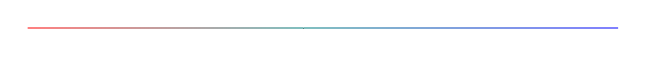
\begin{tikzpicture}
	\fill [left color=red!50, right color=teal!50] (0,0) rectangle (3.5,.01);
	\fill [left color=teal!50, right color=blue!50] (3.5,0) rectangle (7.5,.01);
	\end{tikzpicture}
\vspace{0.5cm}


%%%%%%%%%%%%%%%%%%%%%%%%%%%%%%%%%%%. \begin{ ------>. 
detsacado;  cuadro-naranja;  cuadro-gris;  miejercicio (solución extensa);  mipropuesto (solución corta y fuera del cuadro)

%%%%%%%%%%%%%%%%%%%%%%%%%%%%%%%%%%%. CURIOSIDAD
\vspace{1cm}
\color{ForestGreen!80}
\rule{250pt}{0.2pt}
Texto
\vspace{-8mm}
\begin{flushright}
\rule{250pt}{0.2pt}		
\end{flushright}	
\color{black}
\end{comment}- 